\documentclass[a4paper, 12pt]{article}
\usepackage[T1]{fontenc}
\usepackage[utf8]{inputenc}

\usepackage[a4paper]{geometry}
\usepackage{titlesec}
\usepackage{amsmath}
\usepackage{amsfonts}
\usepackage{amsthm}
\usepackage{xcolor}
\usepackage[bottom]{footmisc}
\usepackage[colorlinks=true, linkcolor=blue, citecolor=red, urlcolor=violet]{hyperref}
\usepackage{graphicx}
\usepackage{subcaption}
\usepackage{caption}


% FIGURES can be defined here and then used or directly defined within the text
\def\FigureOne{\centering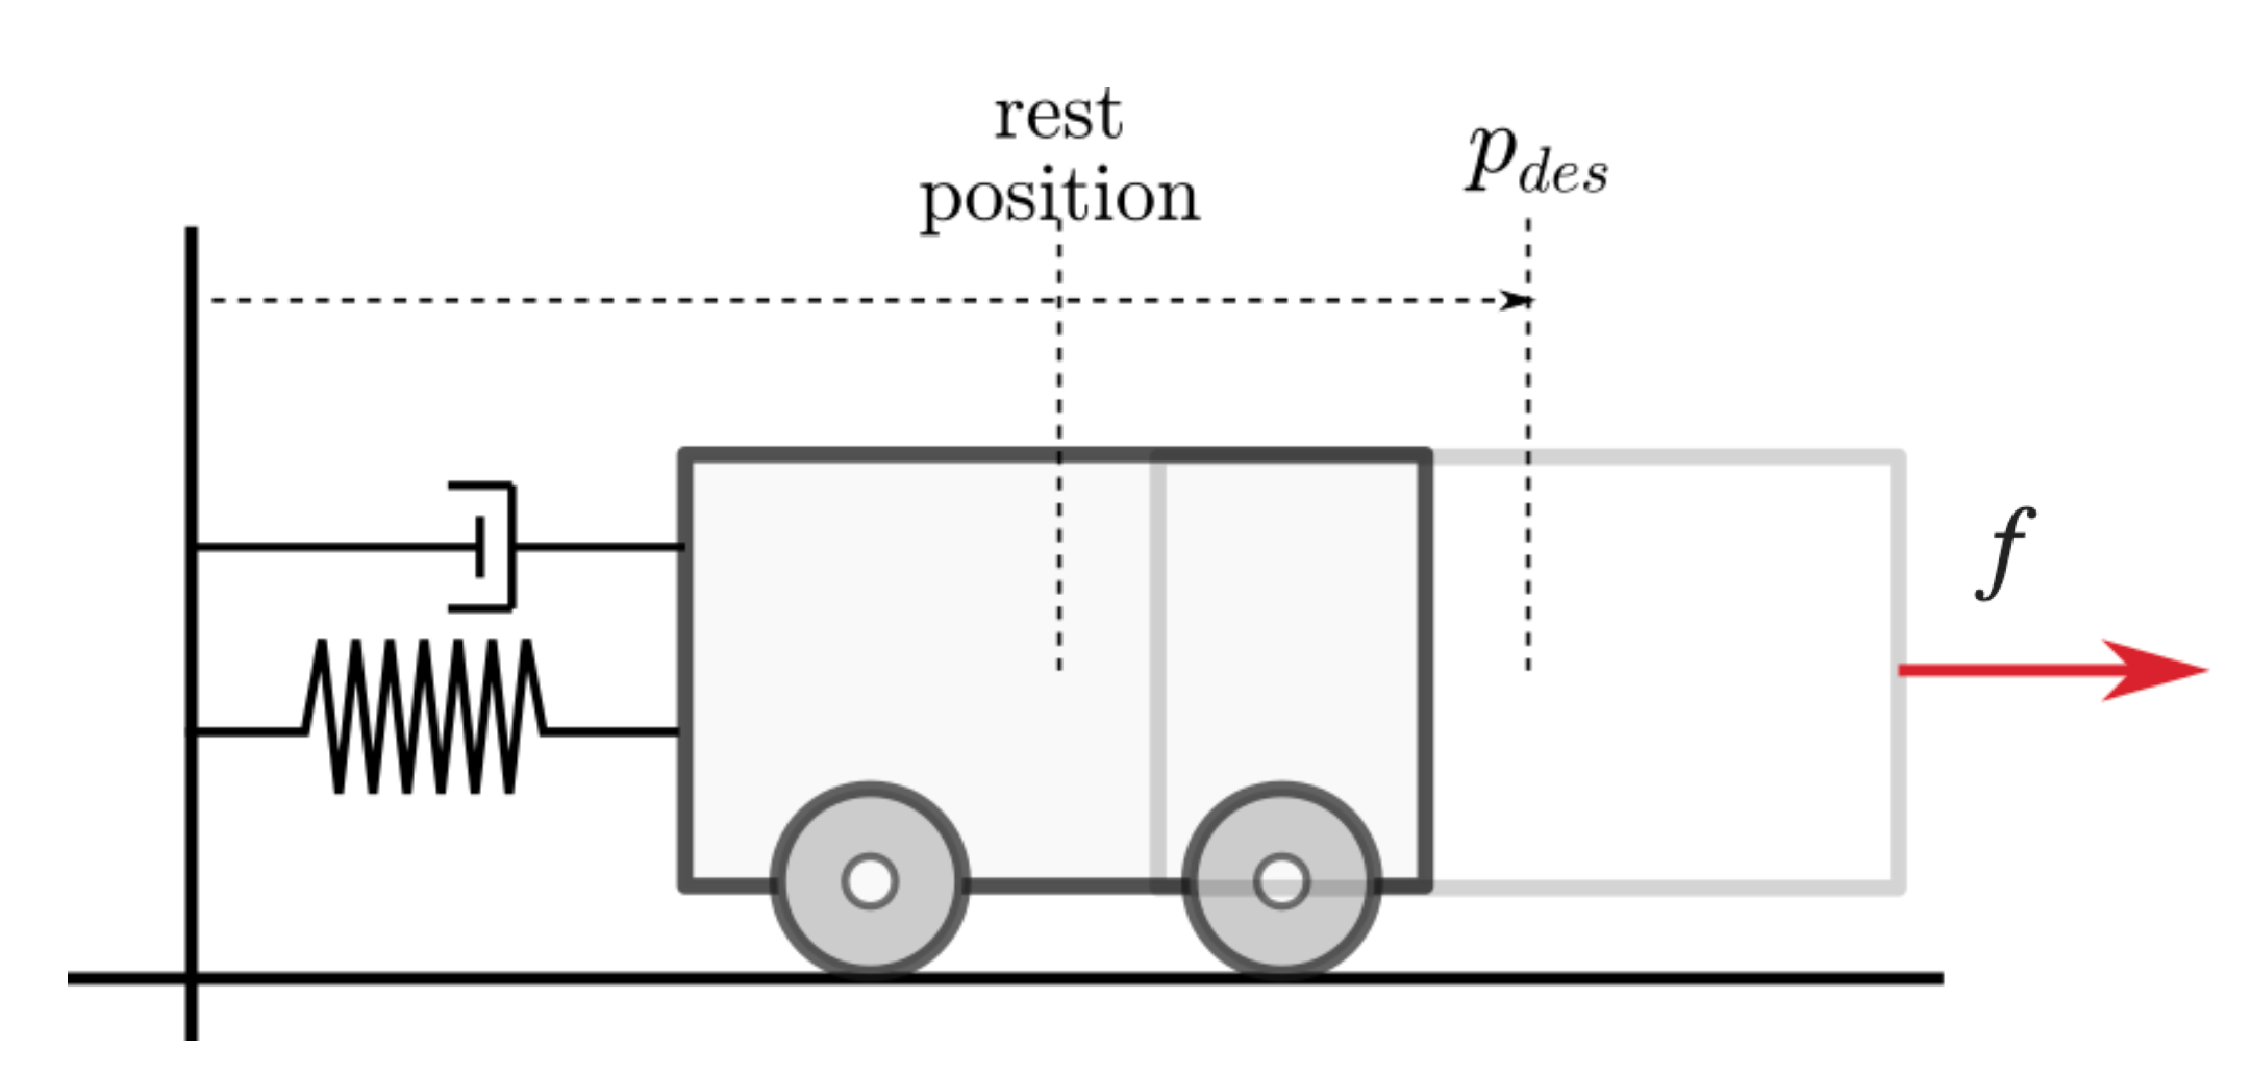
\includegraphics[width=0.5\textwidth]{Figures/fig01.pdf}}

\def\FigureTwo{\centering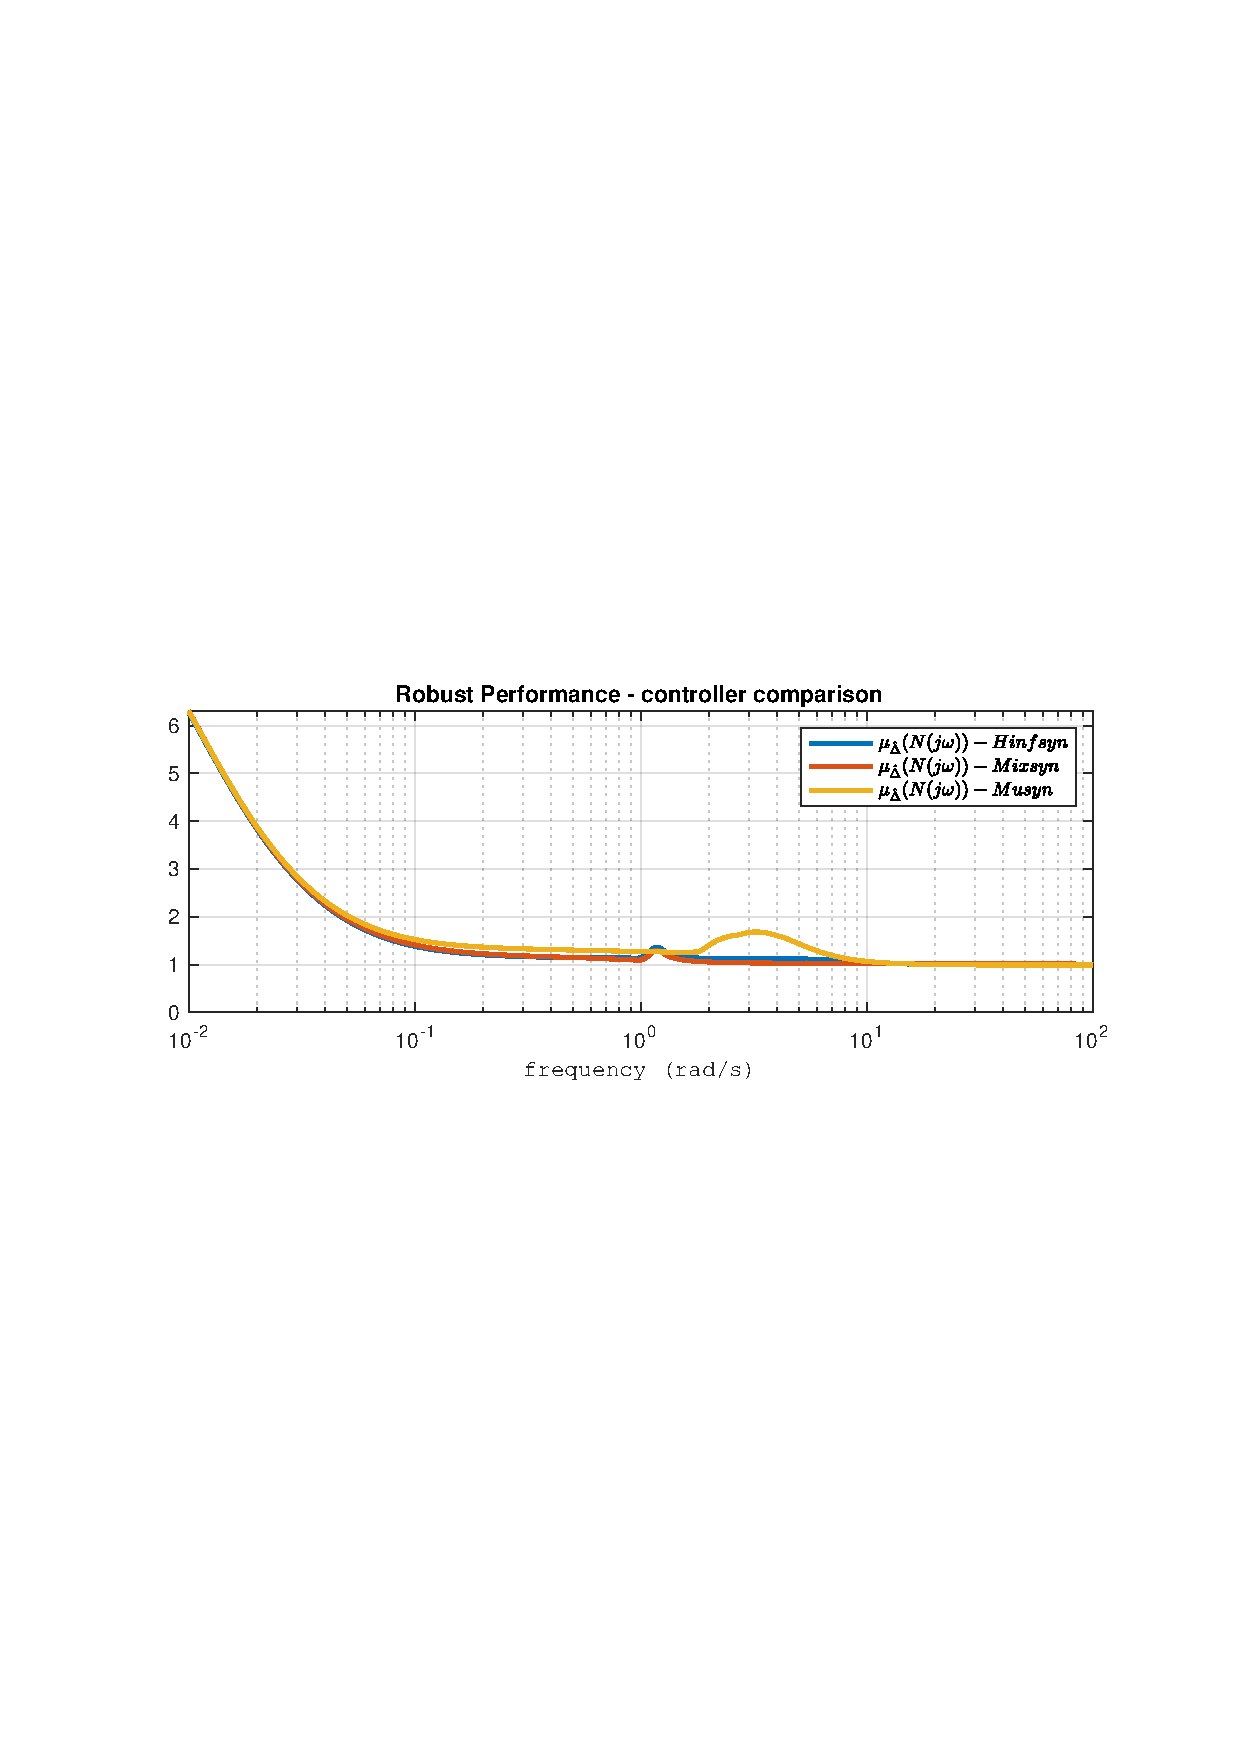
\includegraphics[width=0.8\textwidth]{Figures/fig02.pdf}}
\def\FigureThree{\centering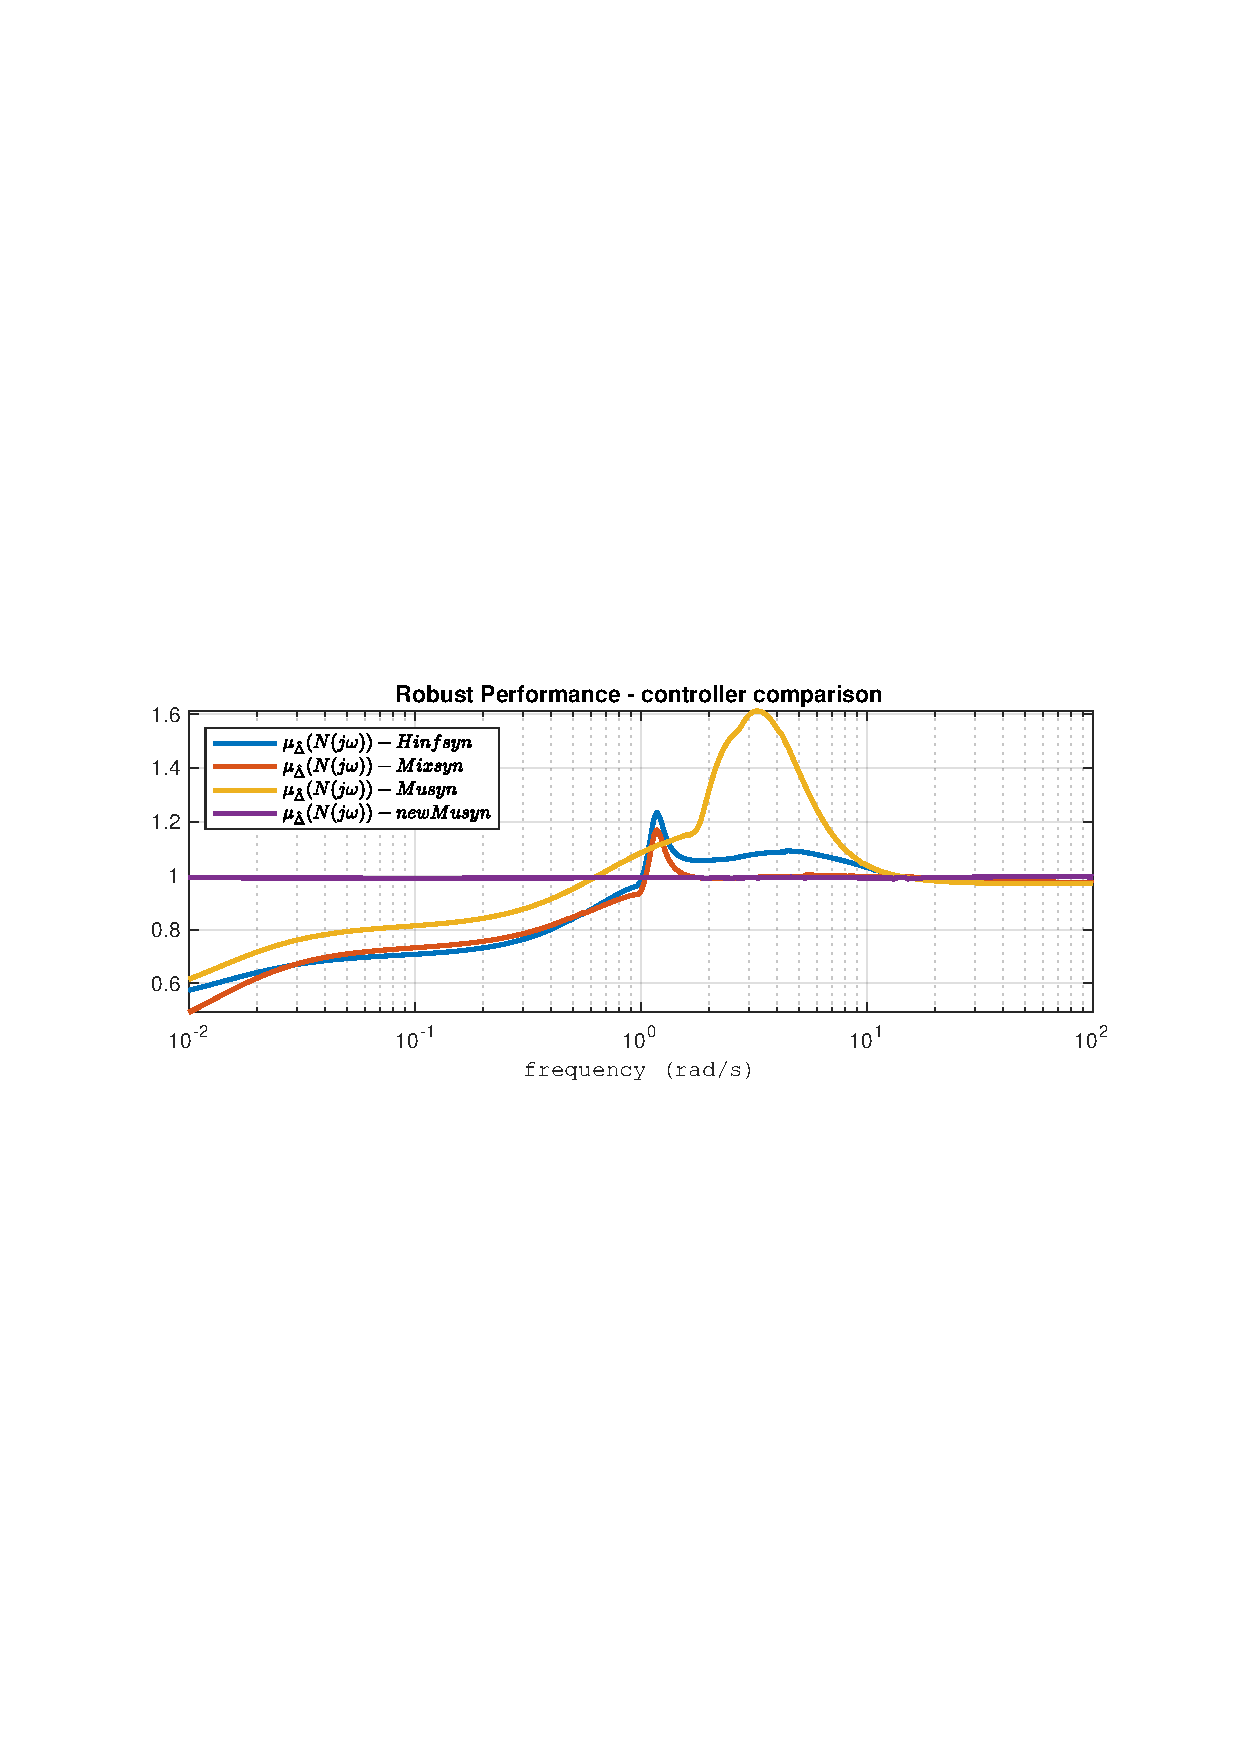
\includegraphics[width=0.8\textwidth]{Figures/fig03.pdf}}

\def\FigureFourA{\centering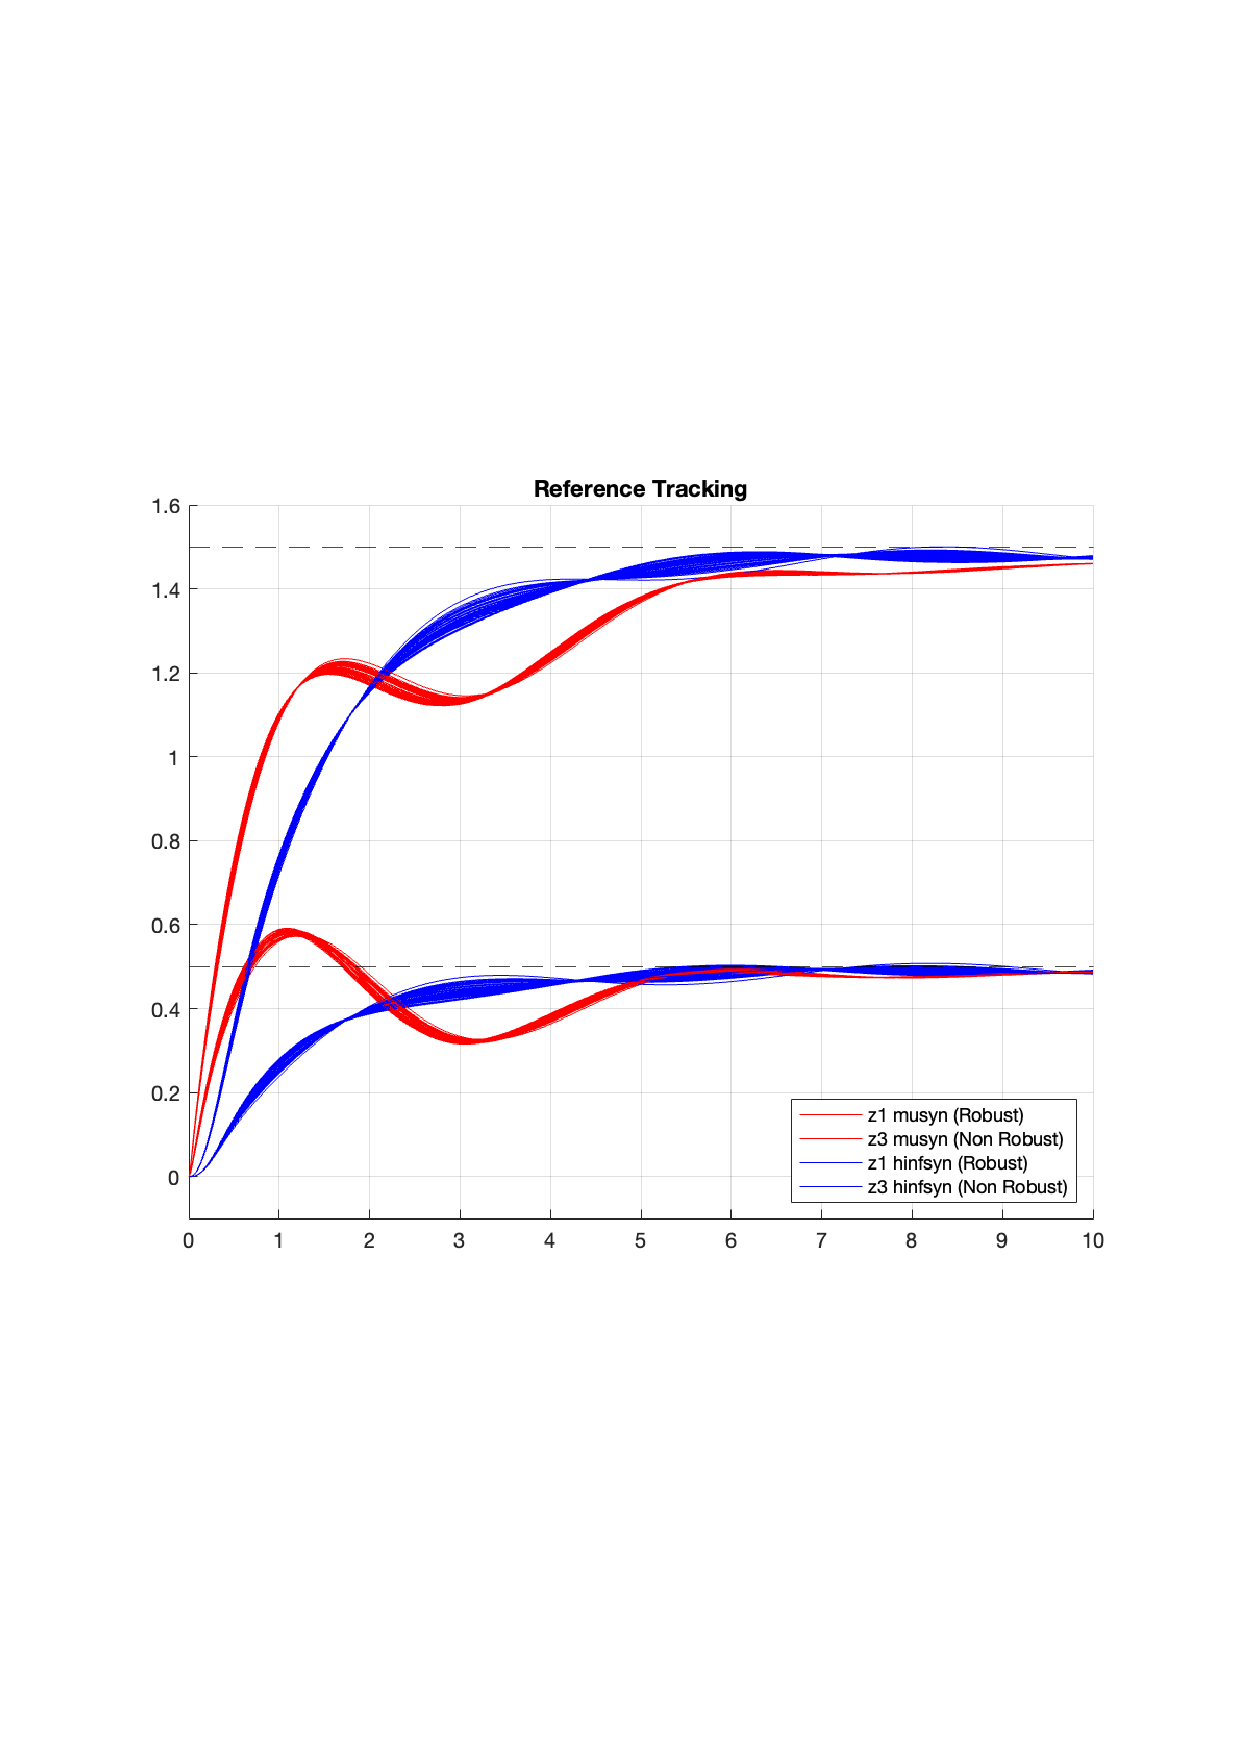
\includegraphics[width=0.45\textwidth]{Figures/fig04a.pdf}}

\def\FigureFourB{\centering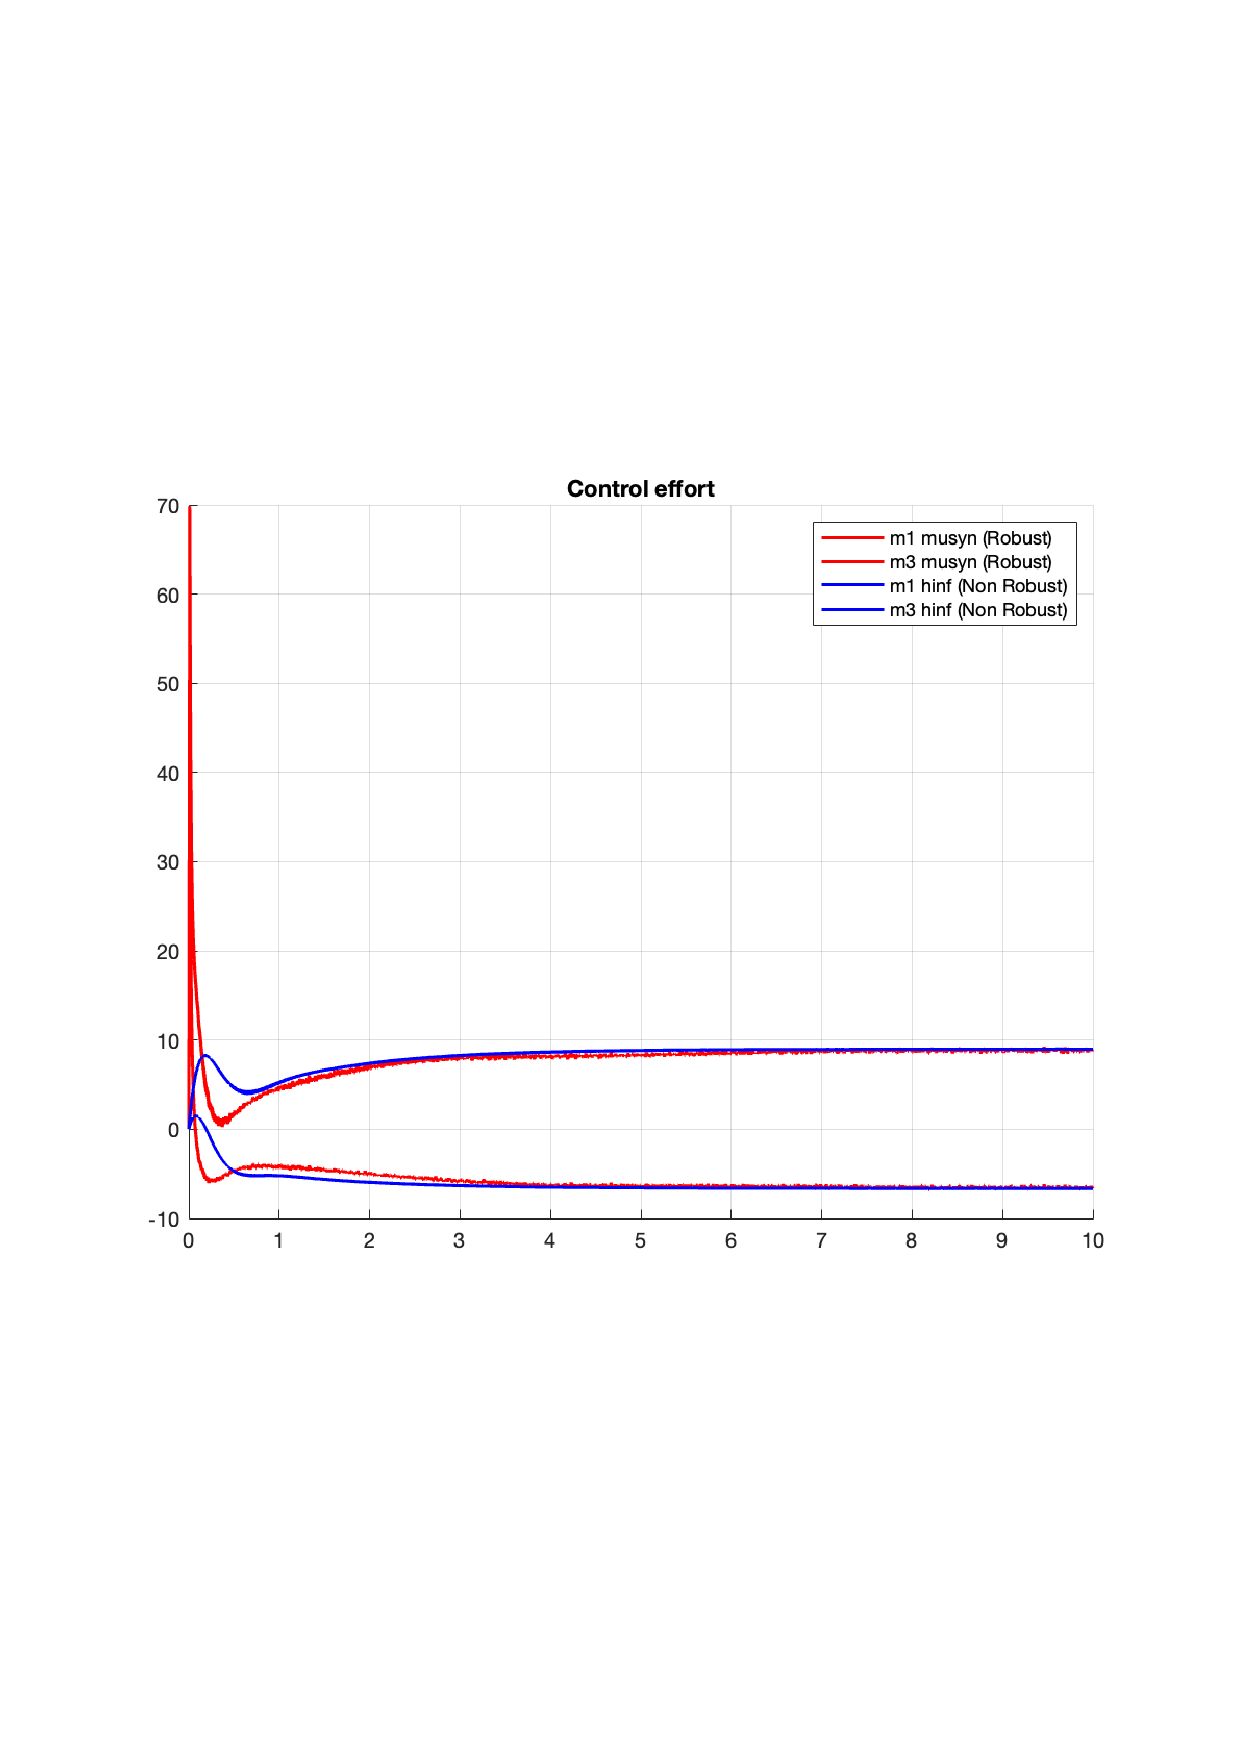
\includegraphics[width=0.45\textwidth]{Figures/fig04b.pdf}}

\def\FigureFive{\centering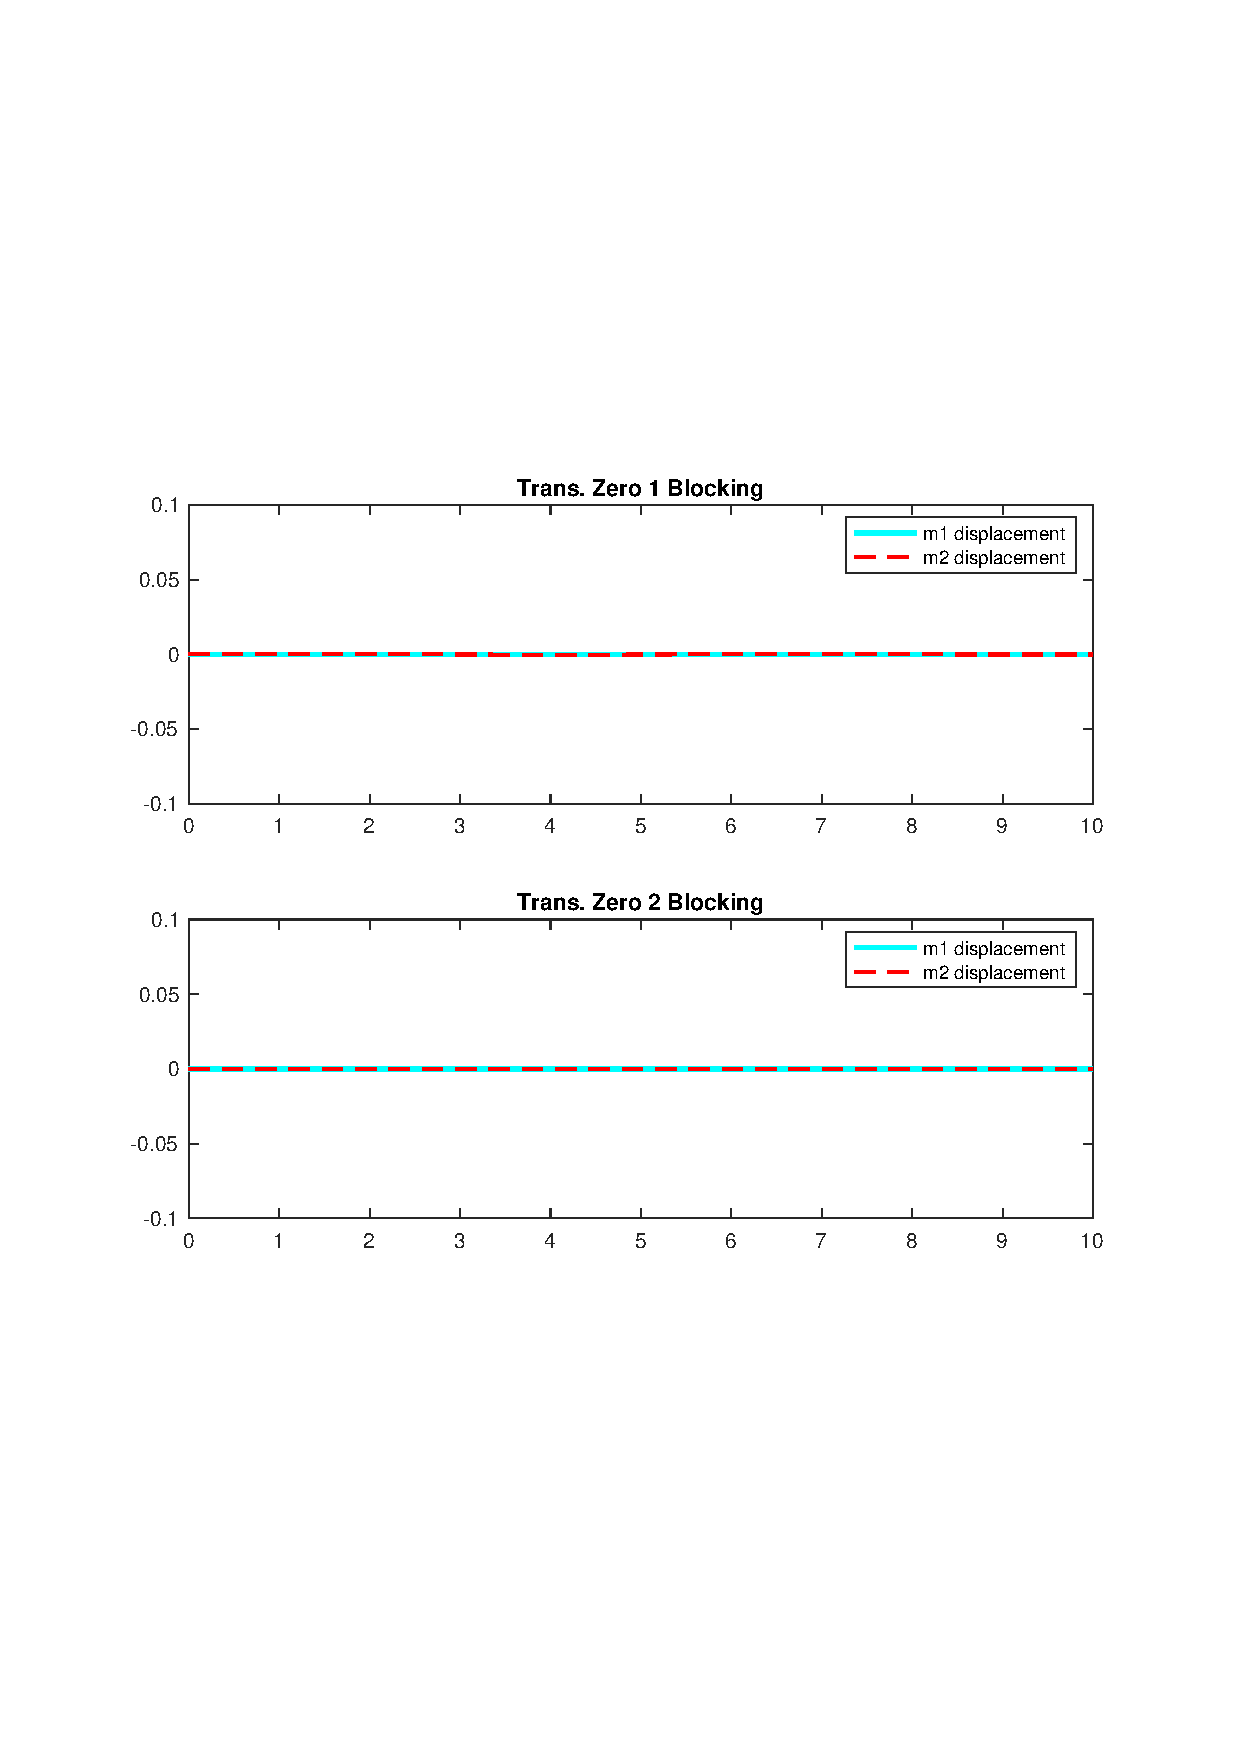
\includegraphics[width=0.8\textwidth]{Figures/fig05.pdf}}

\def\FigureSix{\centering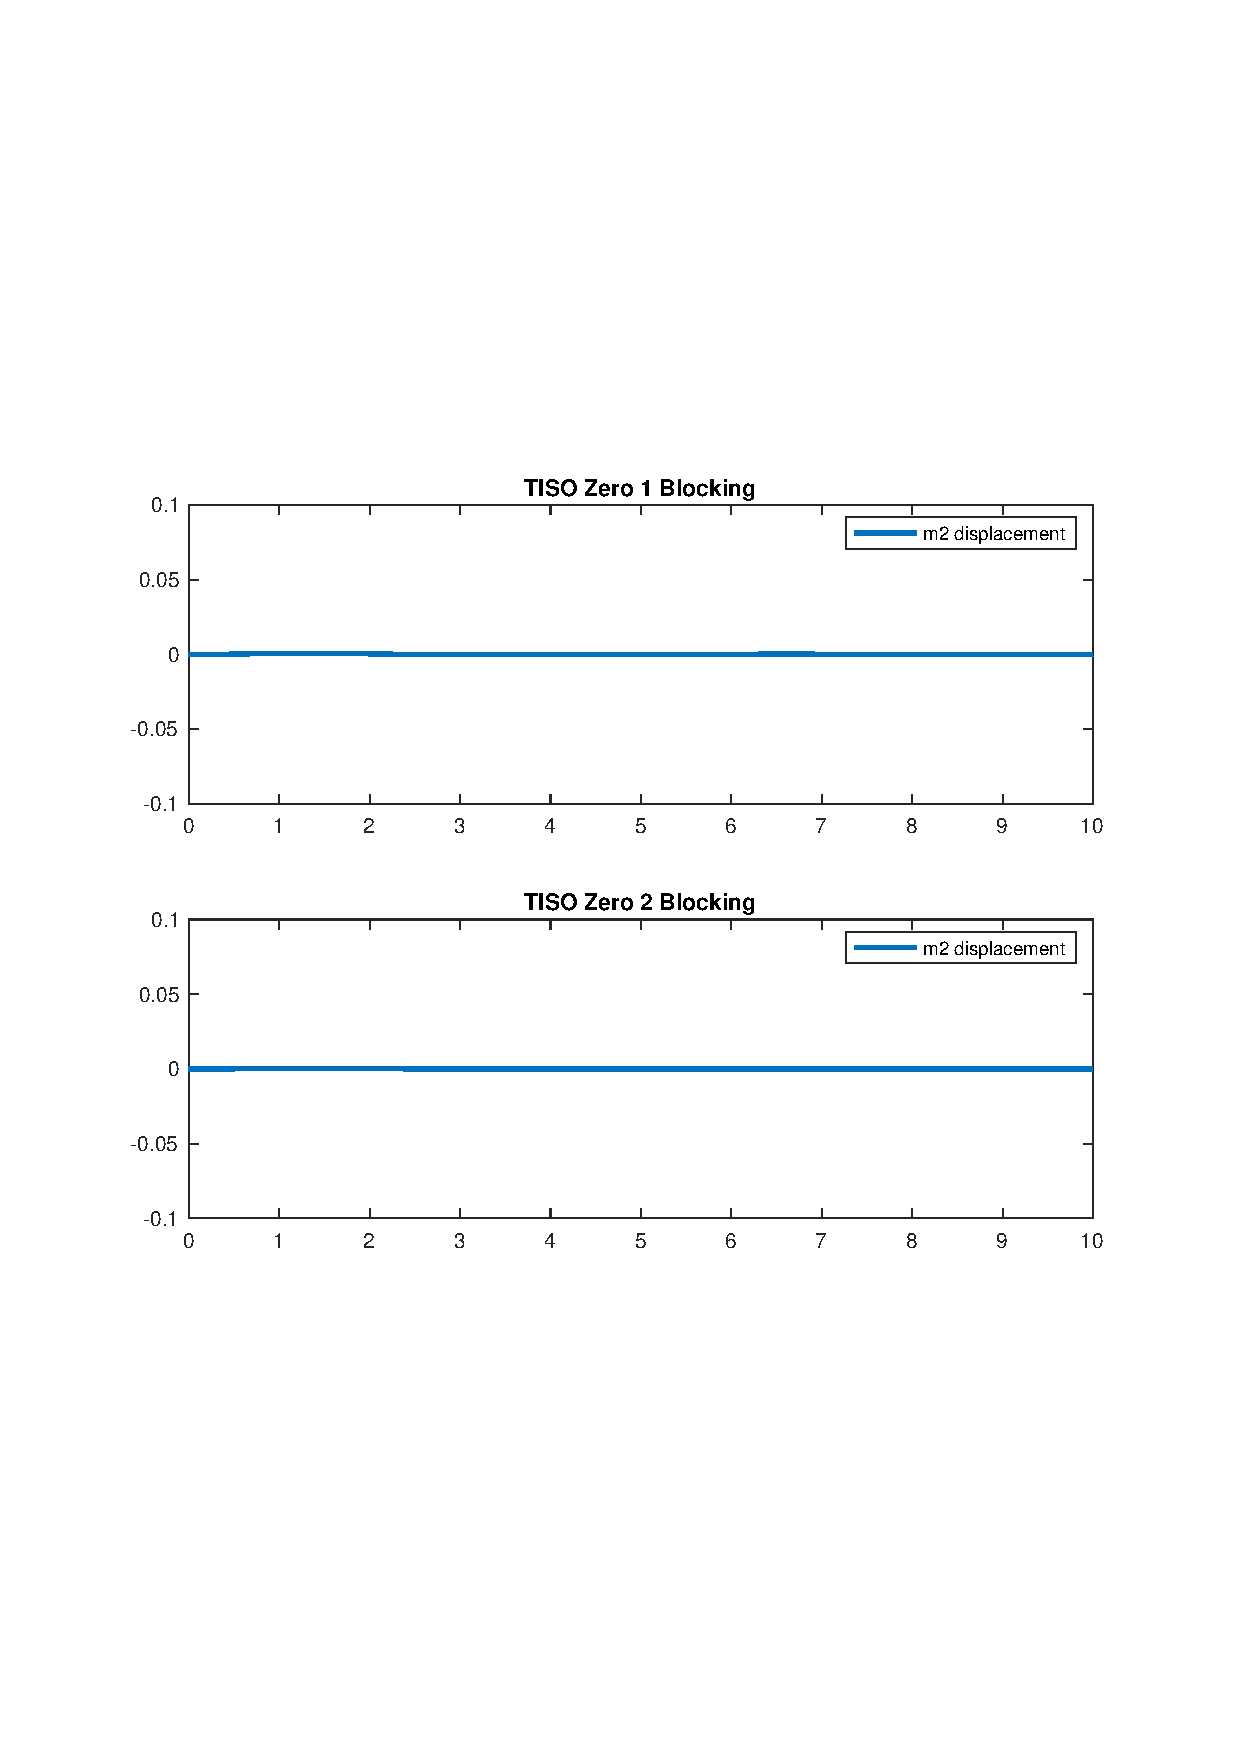
\includegraphics[width=0.8\textwidth]{Figures/fig06.pdf}}

\def\FigureSeven{\centering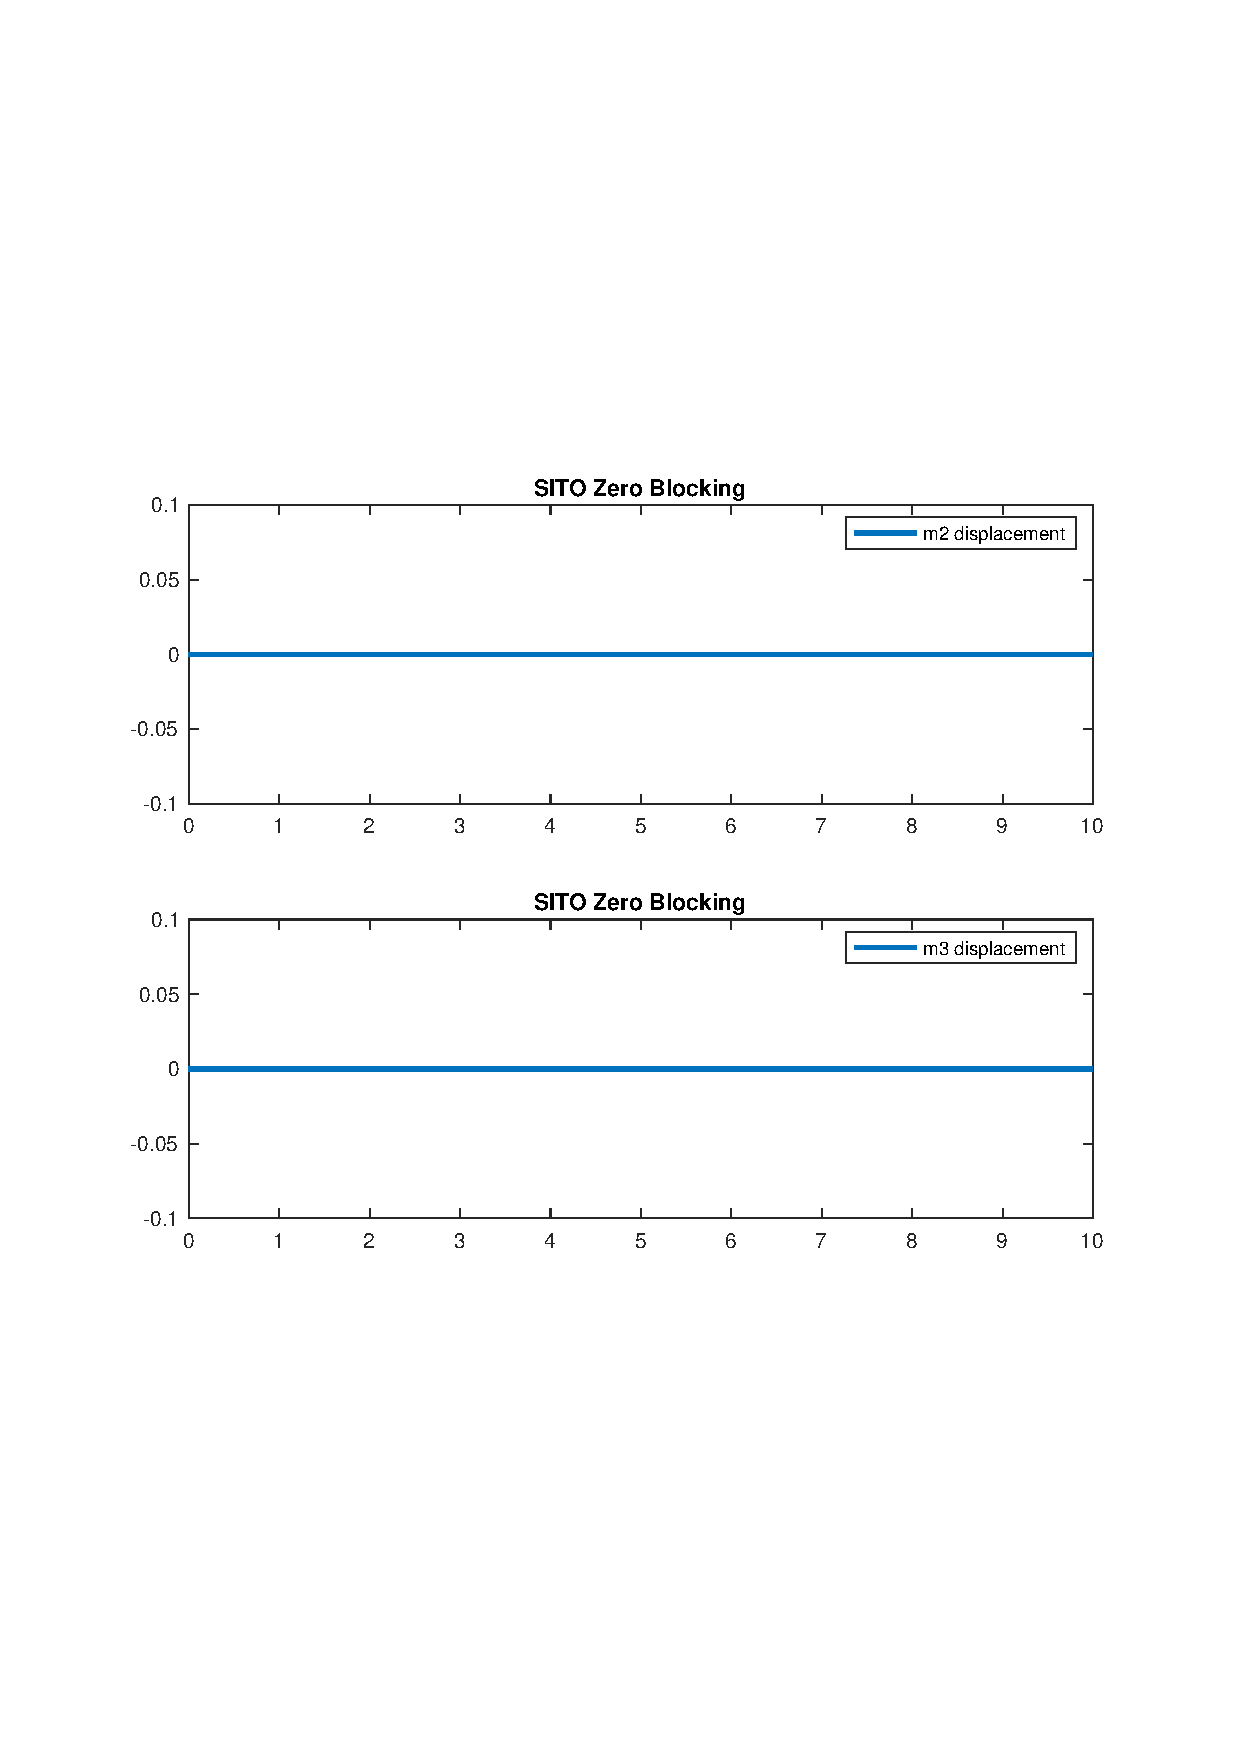
\includegraphics[width=0.8\textwidth]{Figures/fig07.pdf}}

\def\FigureEight{\centering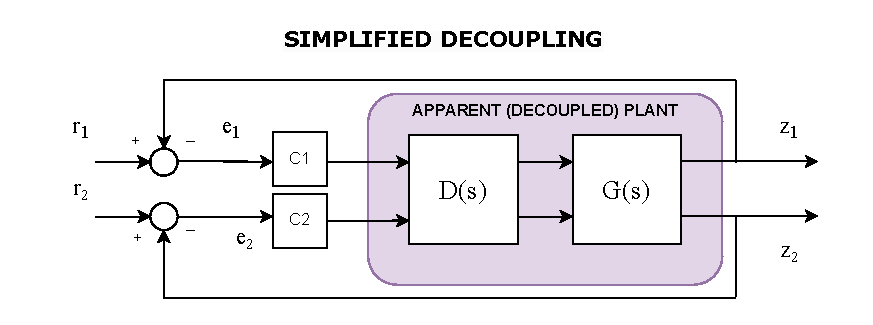
\includegraphics[width=0.6\textwidth]{Figures/fig08.pdf}}

\def\FigureNine{\centering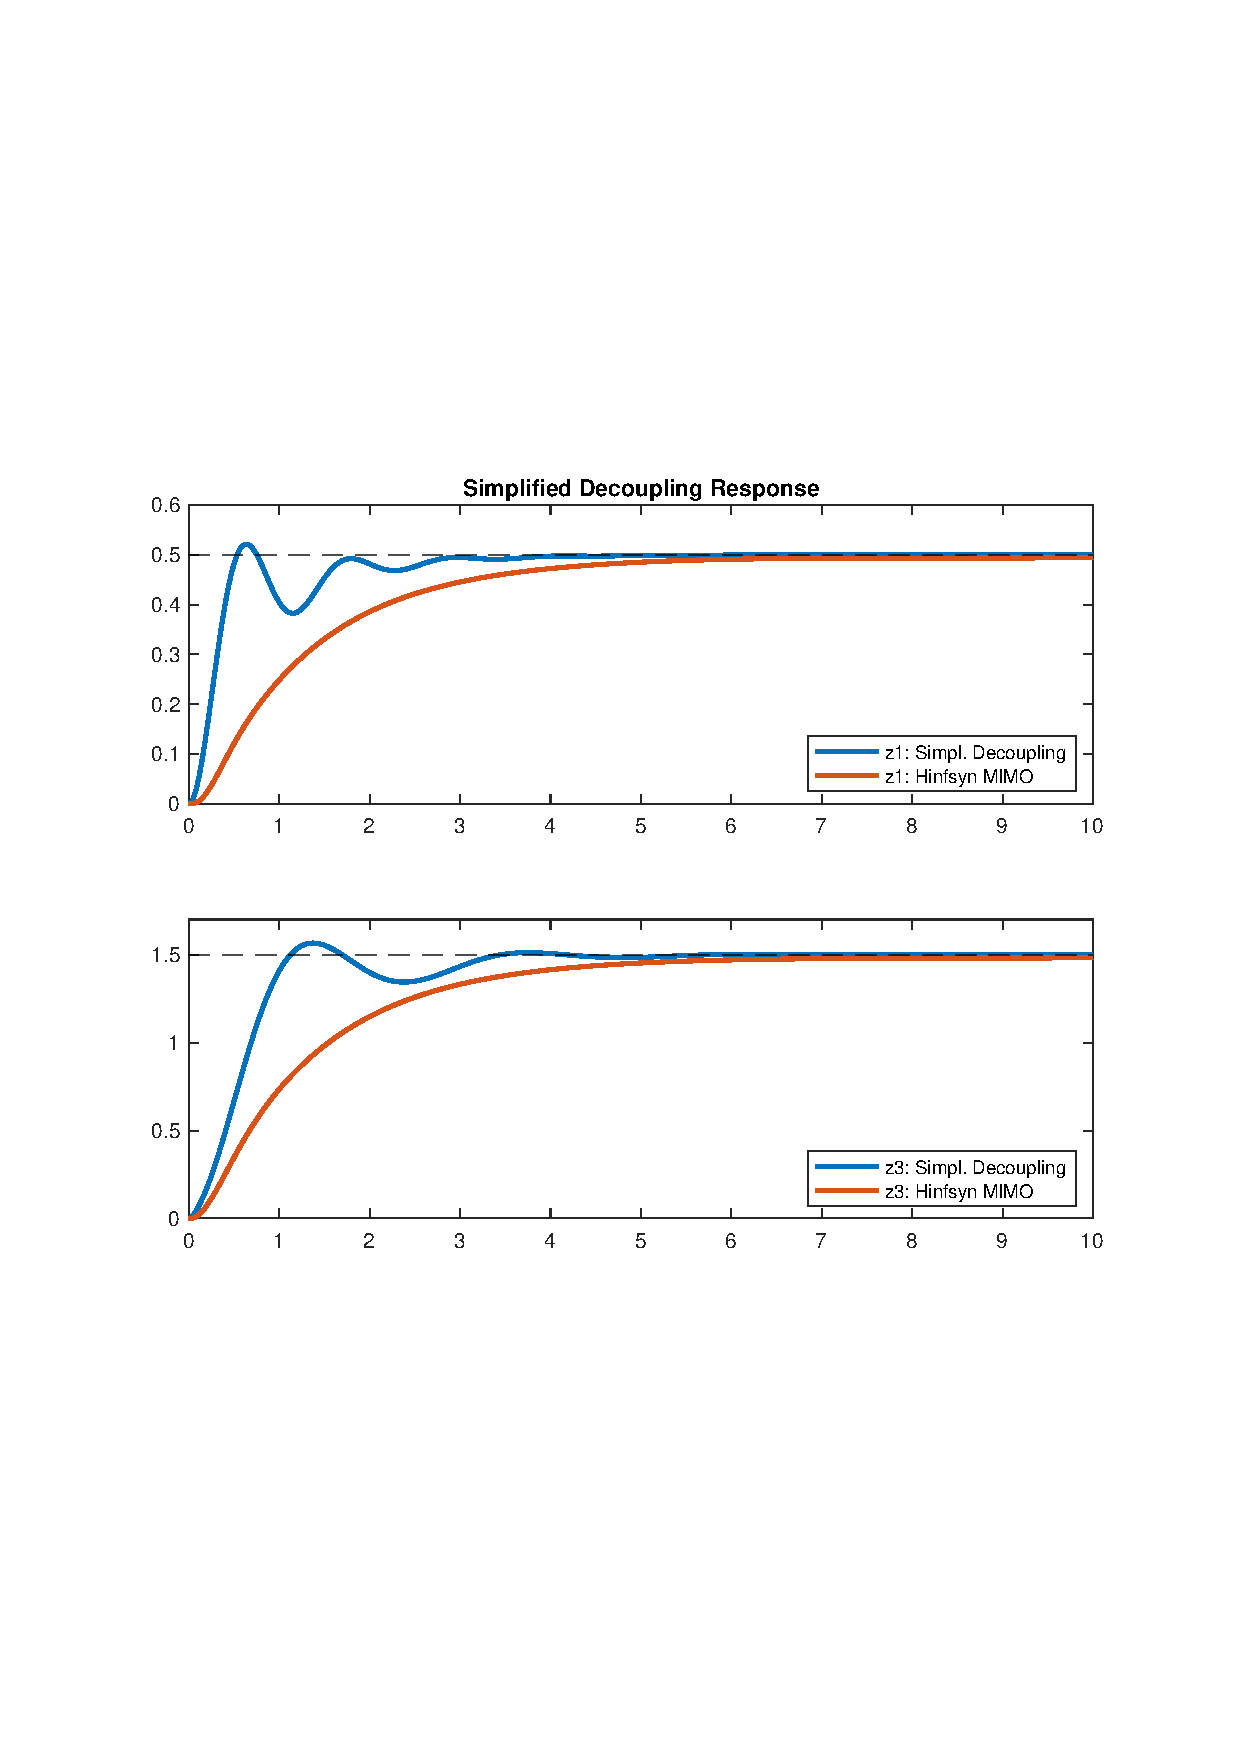
\includegraphics[width=0.6\textwidth]{Figures/fig09.pdf}}

\def\FigureTen{\centering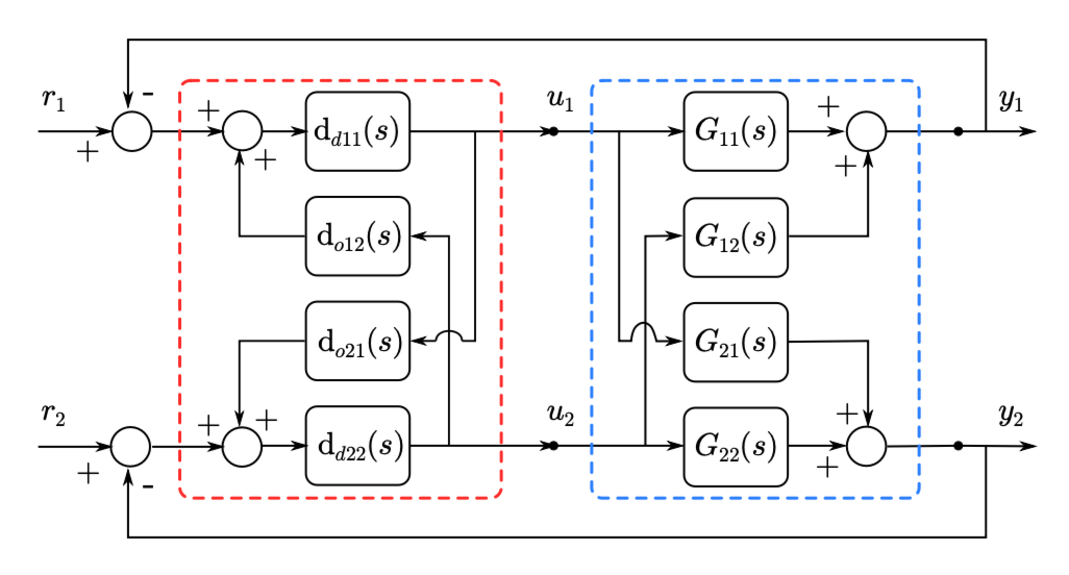
\includegraphics[width=0.6\textwidth]{Figures/fig10.pdf}}

\def\FigureEleven{\centering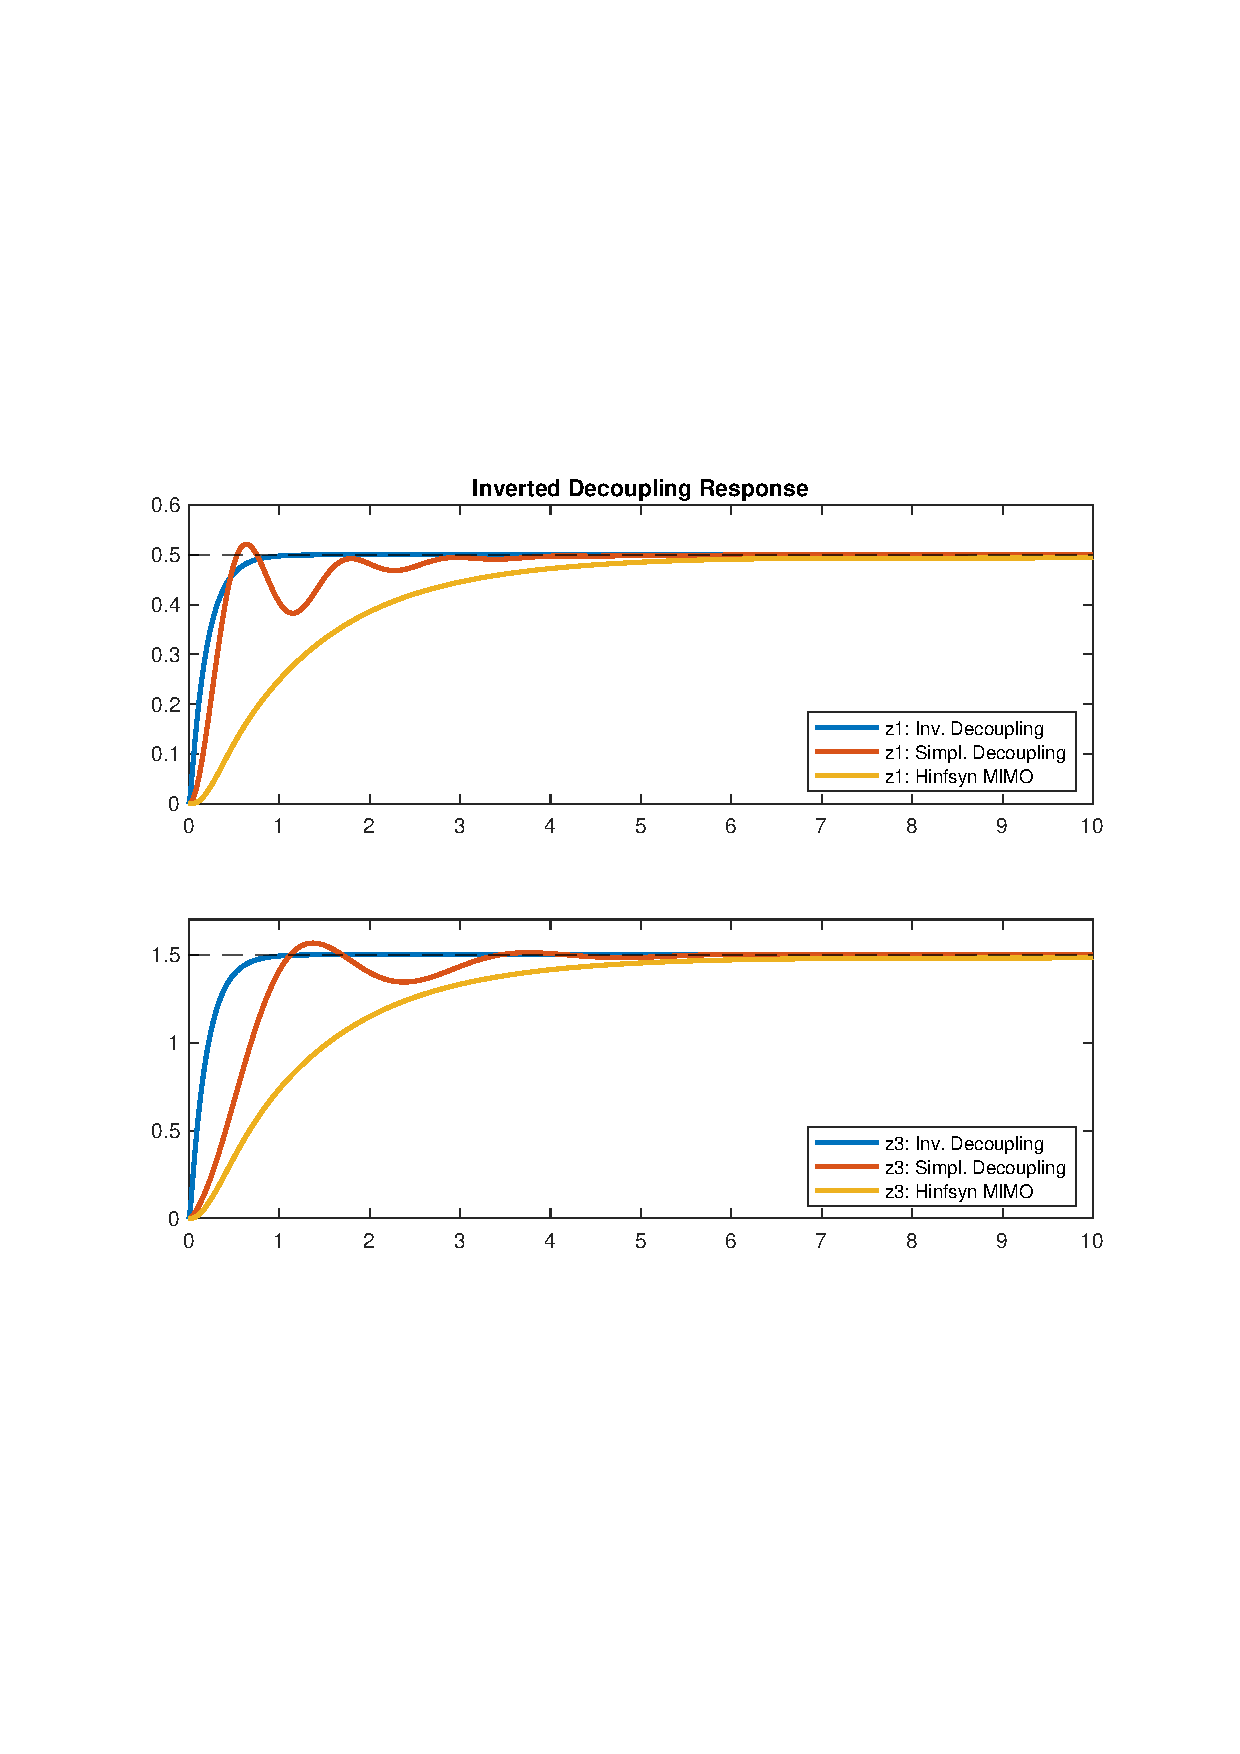
\includegraphics[width=0.7\textwidth]{Figures/fig11.pdf}}

\def\FigureTwelve{\centering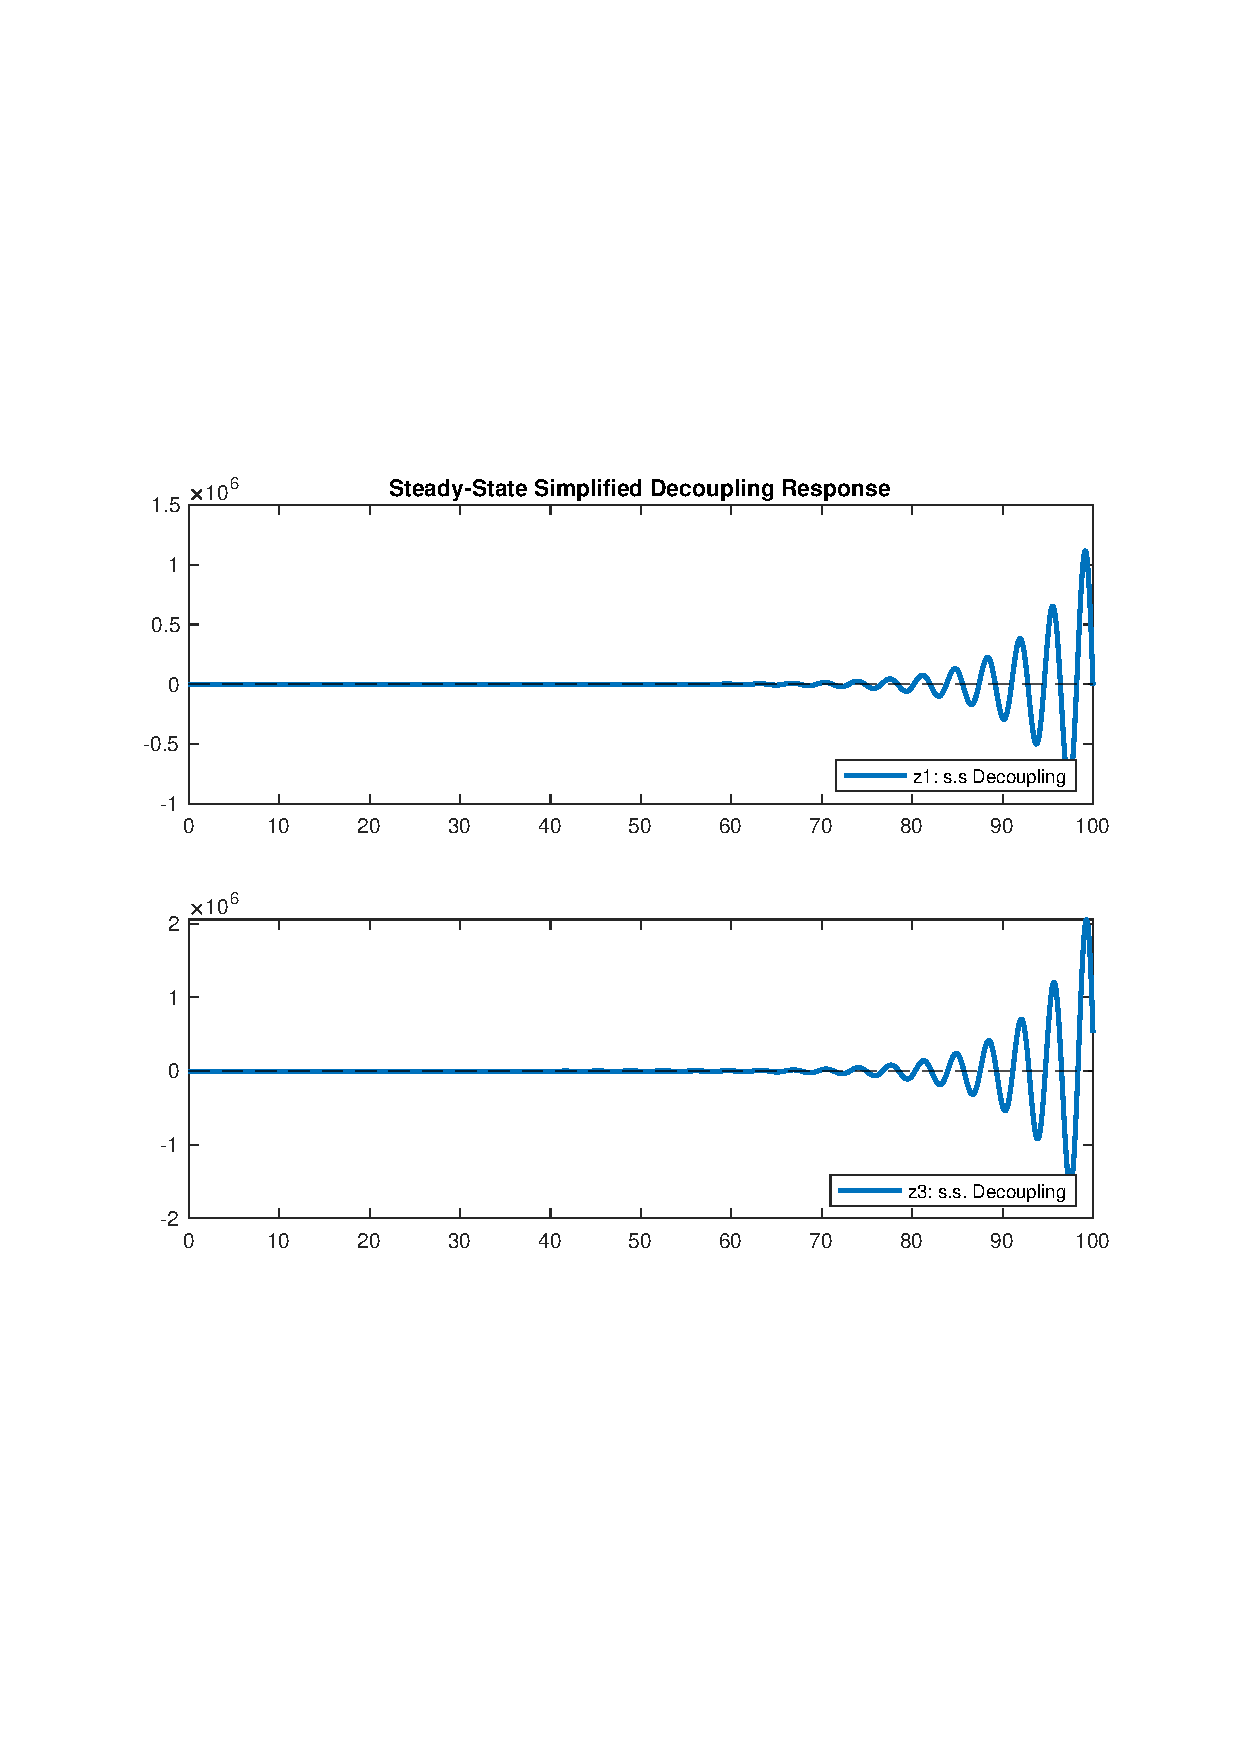
\includegraphics[width=0.7\textwidth]{Figures/fig12.pdf}}

\def\FigureThirteen{\centering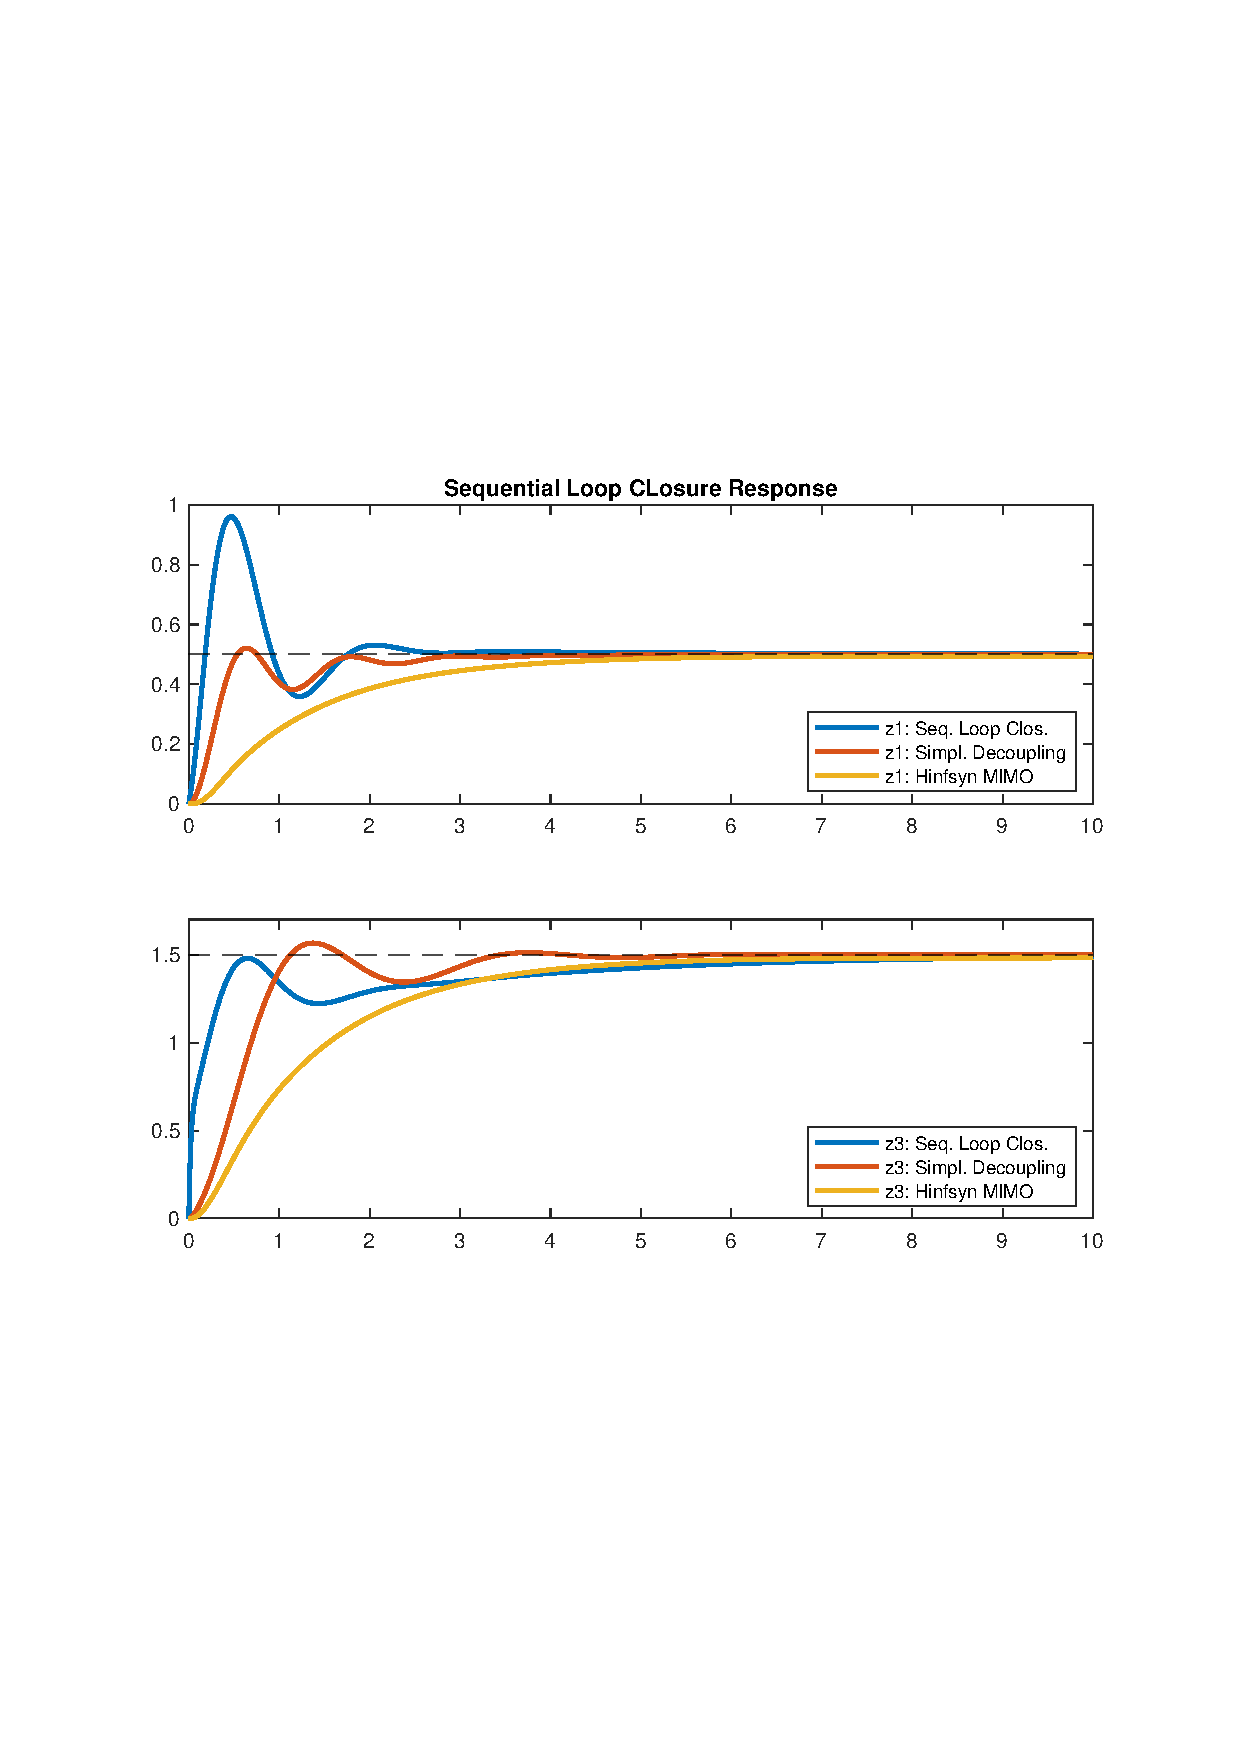
\includegraphics[width=0.7\textwidth]{Figures/fig13.pdf}}

\def\FigureFourteen{\centering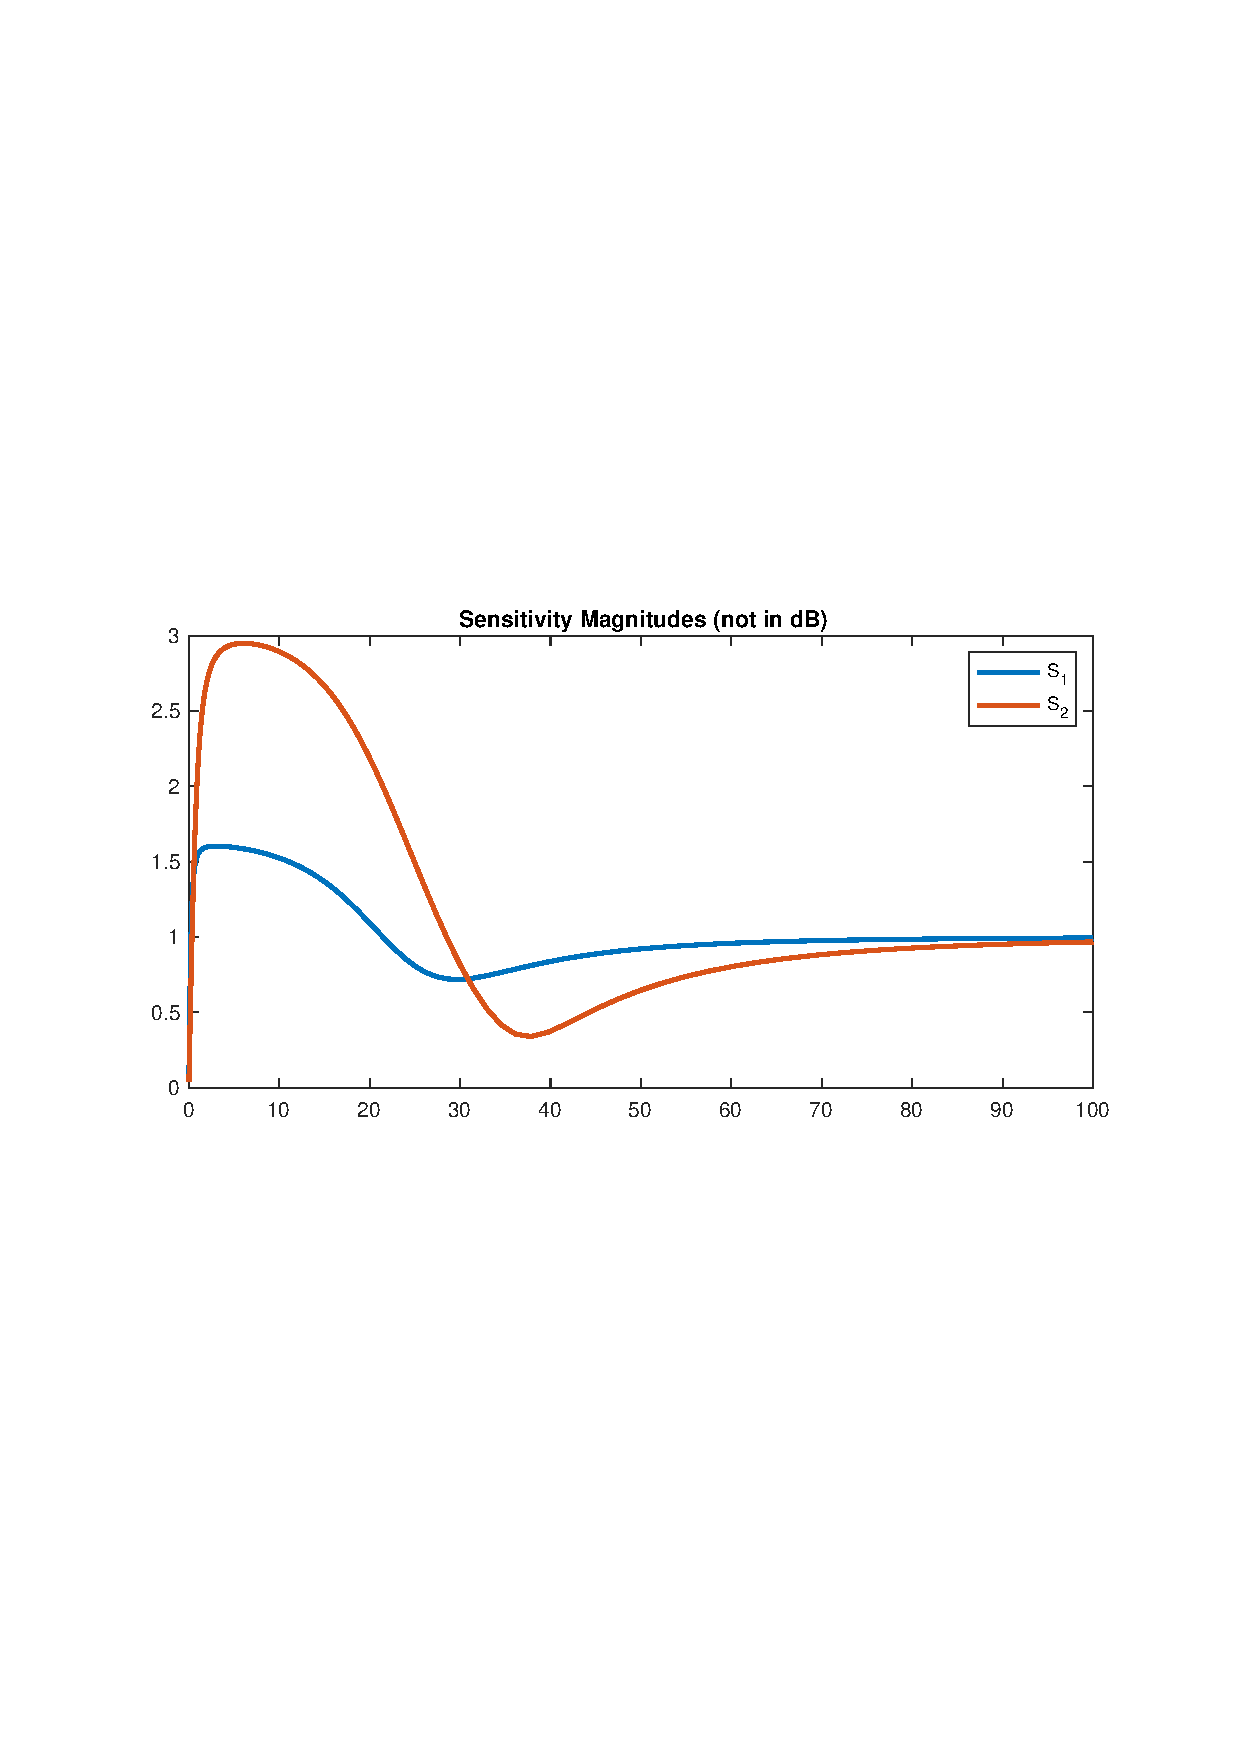
\includegraphics[width=0.6\textwidth]{Figures/fig14.pdf}}

\def\FigureFifteen{\centering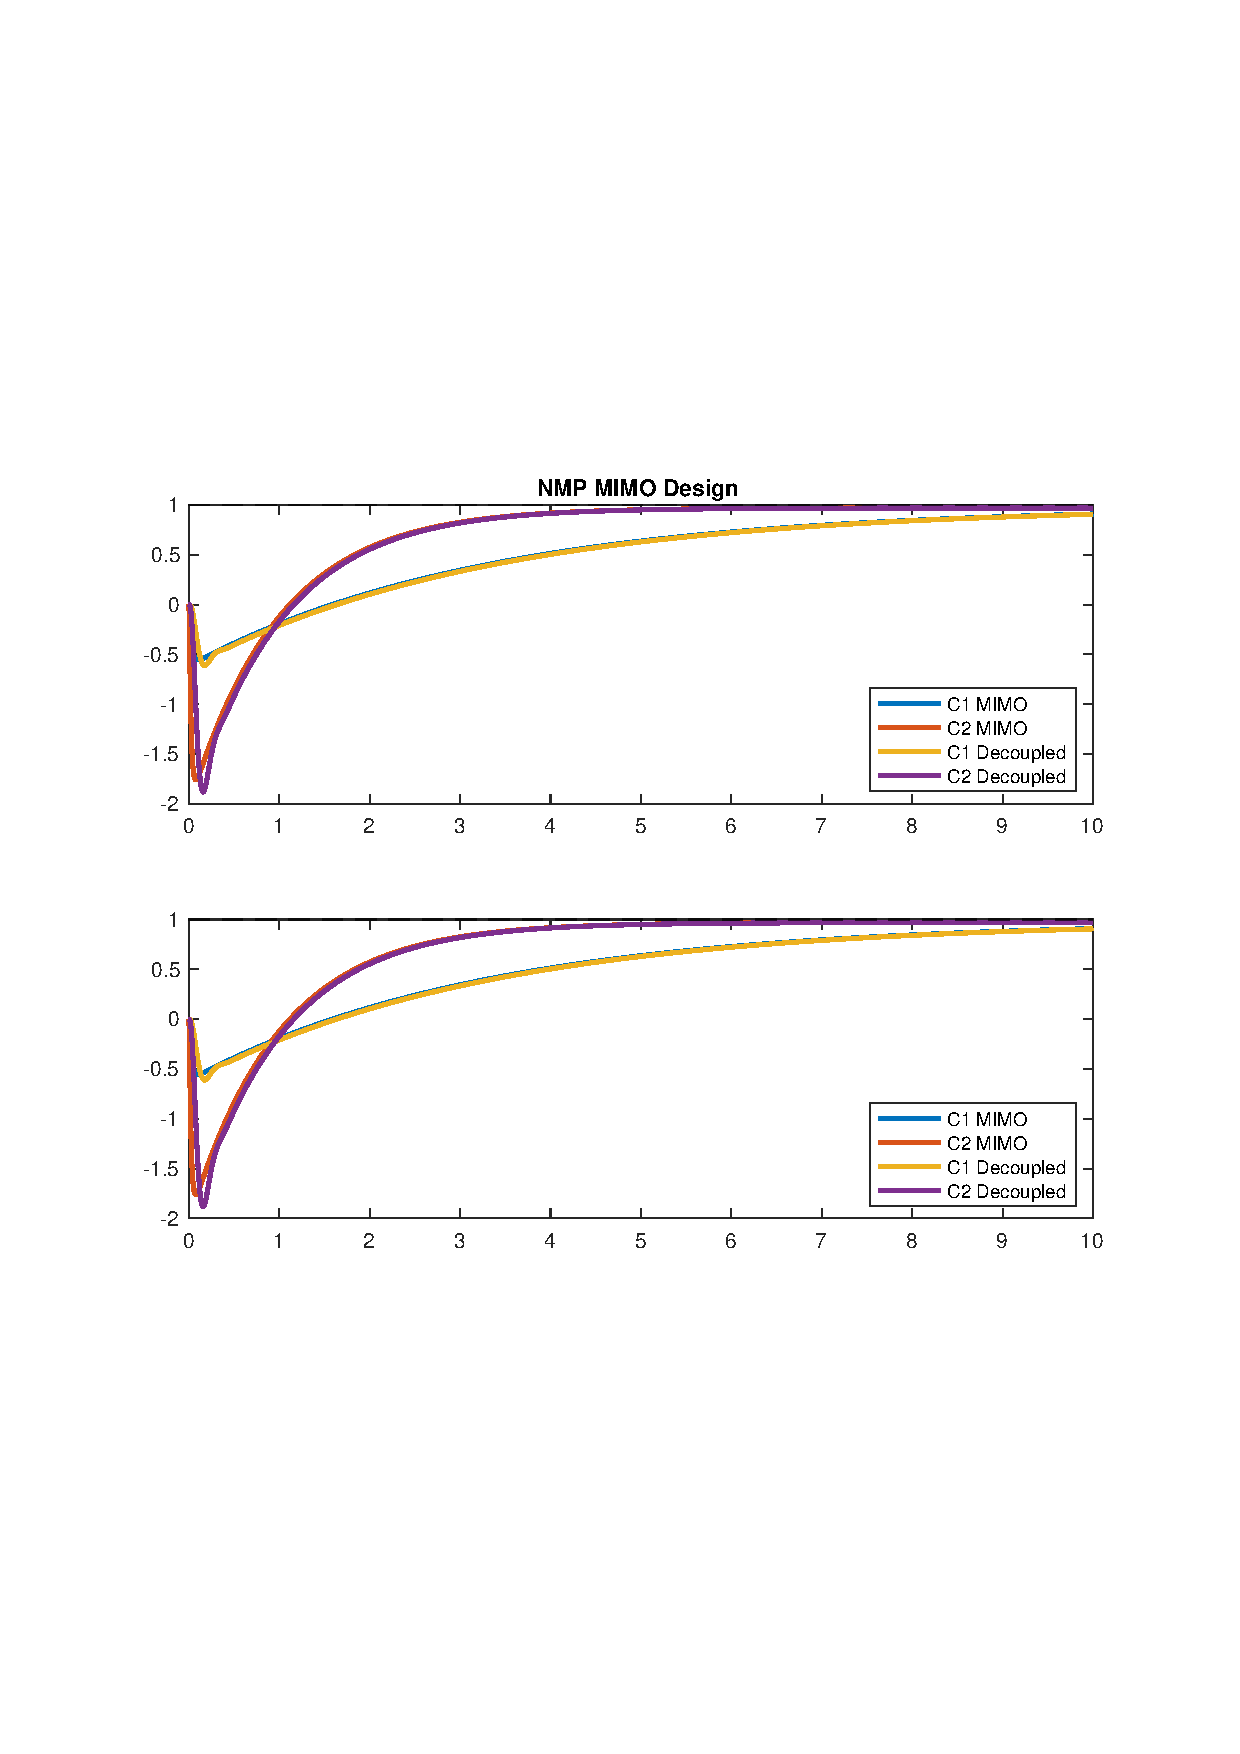
\includegraphics[width=0.9\textwidth]{Figures/fig15.pdf}}

\title{Multivariable Feedback Control \\ Homework 04}
\author{Matteo Scuderi\\ matricola 1937090}
\date{}

\begin{document}

\maketitle
\section{Problem 1: MIMO Robust Performance}
It this section we study robust performance, using the same physical system as in Homework03.
To briefly recap, we want to control the position of the first and third mass and assign them a constant reference, in presence of high frequency measurement noise and a constant disturbance on the first mass.
\begin{figure*}[h!]
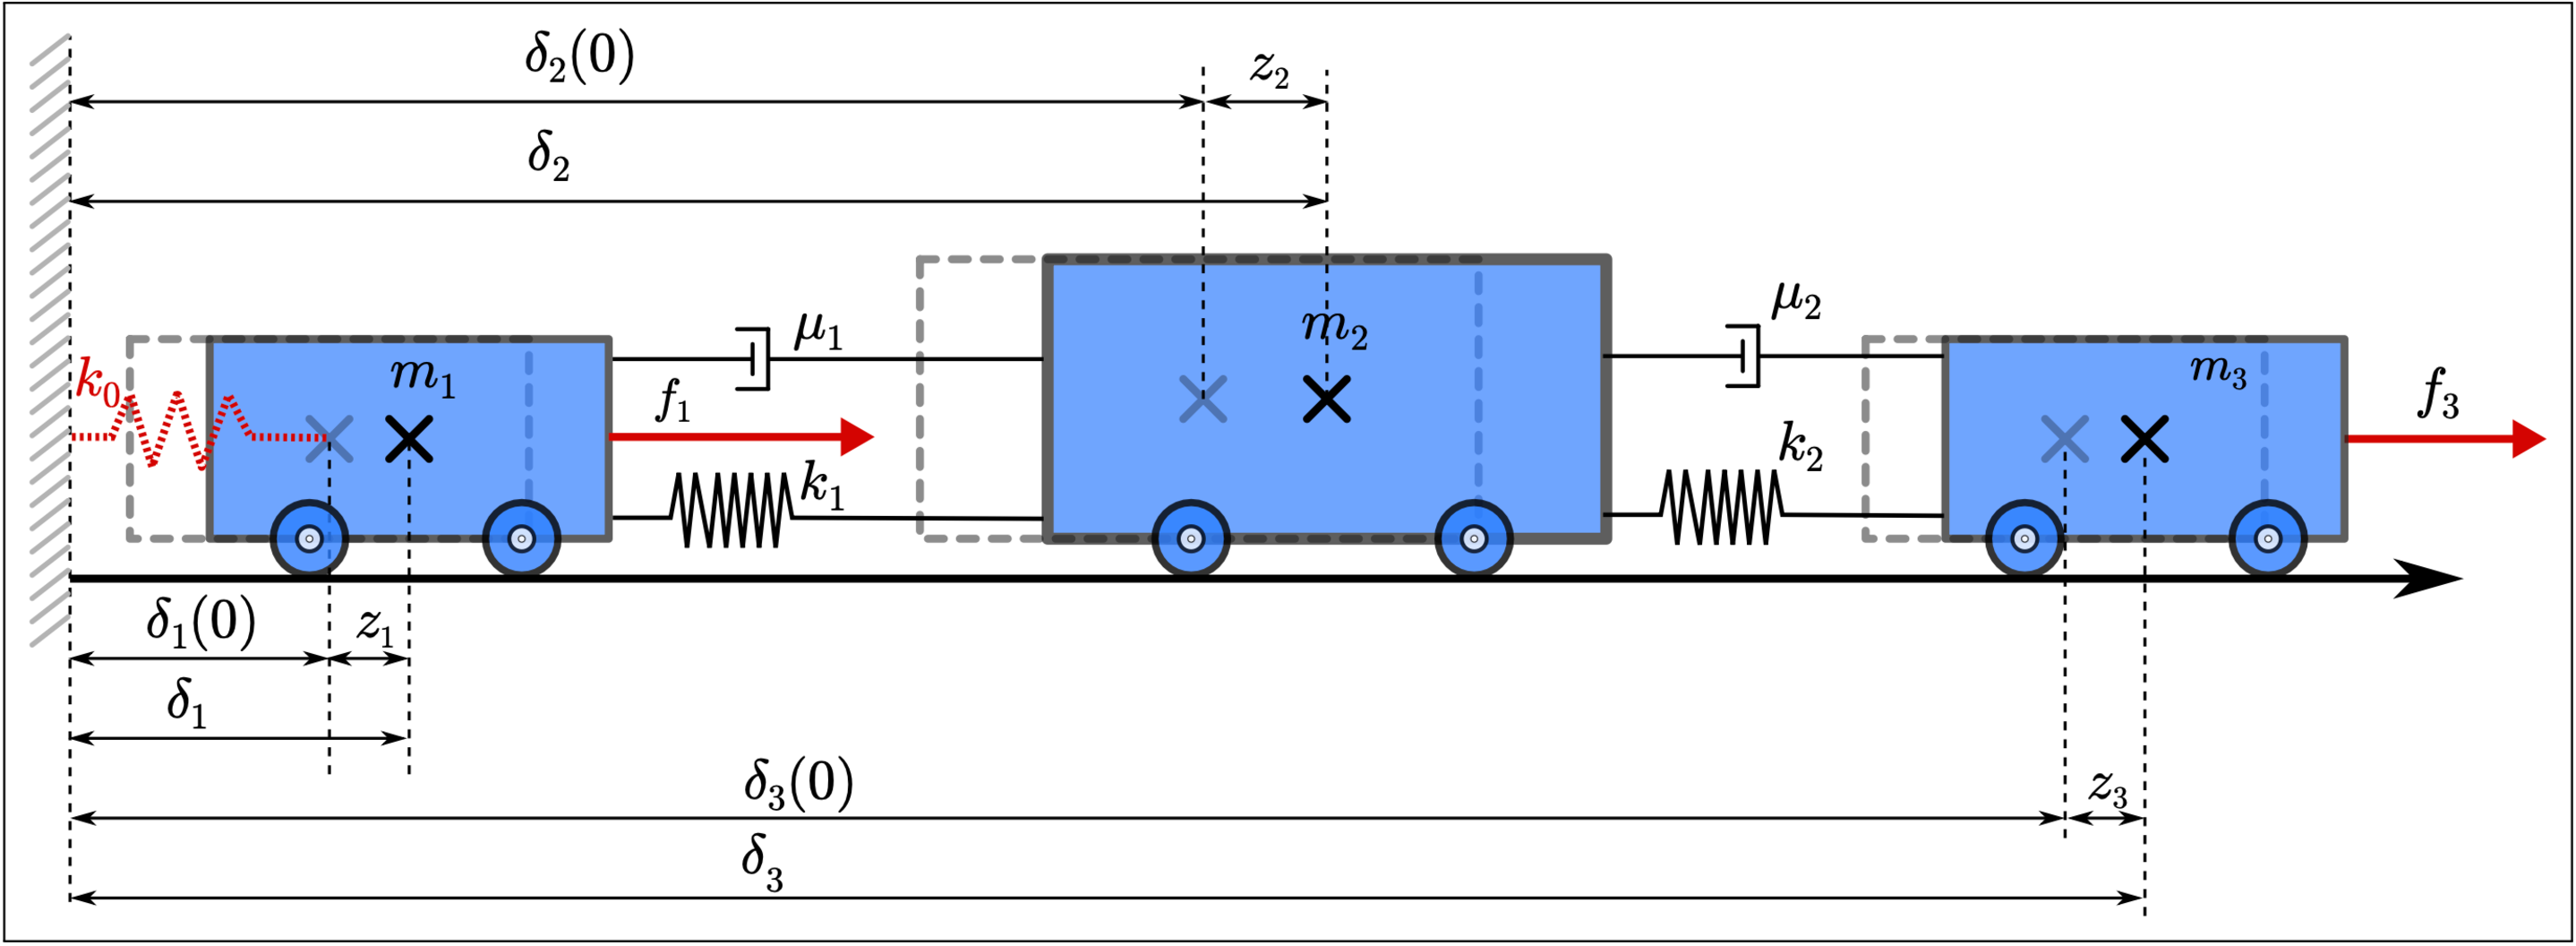
\includegraphics[width=\textwidth]{Figures/3MSD.pdf}
    \caption*{3-MSD System}
\end{figure*}\\
All system's parameters are specified in the Matlab file and for continuity, we'll use the same exact controllers designed in HW03. 
\subsection{$\Delta_F$ formulation "trick"}
Let's take a few steps back to better understand the procedure. 
We have the general uncertain augmented plant, complete with all the performance weights.
\begin{figure}[h!]
    \FigureOne
    \caption{Uncertain G(s) Augmented Plant}
    \label{fig:fig01}
\end{figure}
\\\\ We can than proceed with "pulling out" the uncertainty (using the command $lftdata(...)$). For our system, the uncertainty is a real diagonal matrix \\
$\Delta = \begin{bmatrix}
\delta_1 & 0 & 0\\
0 & \delta_2 & 0\\
0 & 0 & \delta_3
\end{bmatrix}$ in which each $\delta_i$ term represents the uncertainty of the $m_i$ mass and is such that $\|\delta_i(j\omega)\|_\infty < 1$. 
\\\\
The obtained control scheme can be visualized as the following:
\begin{figure*}[h!]
\centering
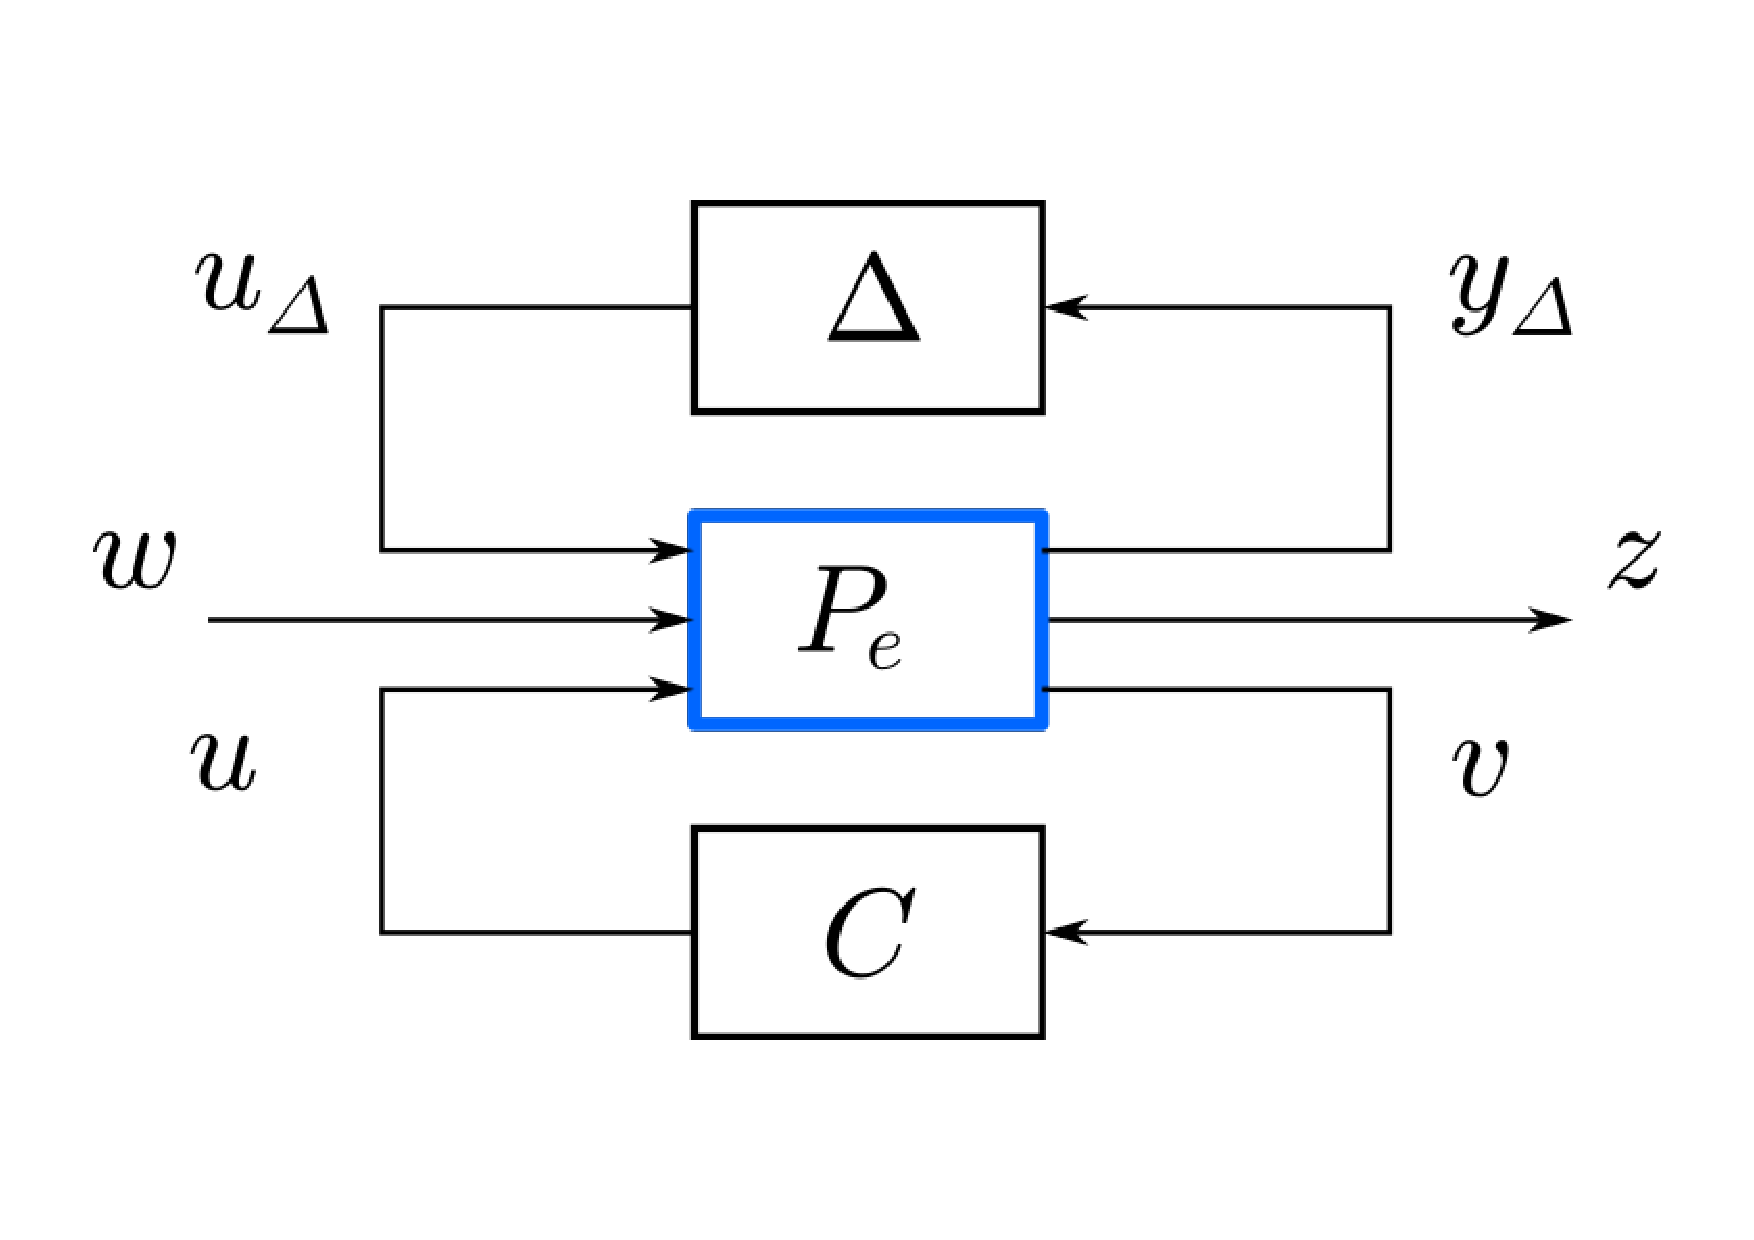
\includegraphics[width=0.5\textwidth]{Figures/extra01.pdf}
\end{figure*}\\
We can now proceed with closing the controller loop with the lower lft and consider the resulting $N = F_\ell (P_e,C)$. \\
To check robust performance, we consider a "fake" extra, full complex uncertainty $\Delta_F$, so that the total uncertainty matrix becomes:
\\$\hat{\Delta} = \begin{bmatrix}
\delta_1 & 0 & 0 & 0\\
0 & \delta_2 & 0 & 0\\
0 & 0 & \delta_3 & 0 \\
0 & 0 & 0 & \Delta_F
\end{bmatrix}$ with $dim(\Delta_F) \equiv dim(N_{22})$.
\\
We can now use this structured, "extended" uncertainty $\hat{\Delta}$ to ensure robust performance, which is guaranteed if $\mu_{\hat{\Delta}}(N) < 1$ 
\subsection{Robust Performance Analysis}
As previously mentioned, we'll check robust performance on all the controllers designed in HW03.
\\
Unfortunately, none of the controllers above, tested on the augmented Plant in Fig.~\ref{fig:fig01} (considering $N = F_\ell (P_e,C)$), achieves robust performance. In particular, the weights considered are the same used for $myxsyn(),hinfsyn(),musyn()$ design in HW03 and can be found in the Matlab file.
The plots $\mu_{\hat{\Delta}}(N)$ for each controller are reported below.
\begin{figure}[h!]
    \FigureTwo
    \caption{$\mu_{\hat{\Delta}}(N)$ >> 1 for some \omega, for all controllers}
    \label{fig:fig11}
\end{figure}
\\Clearly, all plots significantly exceed the 1 bound, proving that robust performance is not ensured.
\subsection{Robust Performance Design}
Let's try to design a new controller that can achieve robust performance. Clearly, the performance weights chosen are too demanding with respect to the system's uncertainty.\\
We'll therefore sacrifice a bit of "performance demand" in choosing the new weights and try to use $musyn(\dots)$ on the usual control scheme. 
\\ In particular, we're going to sacrifice bandwidth, steady state tracking error and maximum control effort. \\Once again, the exact performance weights are left in the Matlab file.
\subsubsection{SSV for the new Augmented Plant}
We can consider now the new augmented plant, which differs from the previously used one only for its weights.
\\
Using the same "$\Delta_F$ trick", we consider $N = F_\ell (P_e^{\ new},C)$ and check its $\mu_{\hat{\Delta}}(N)$.

\begin{figure}[h!]
    \FigureThree
    \caption{$\mu_{\hat{\Delta}}(N)$ < 1 only for the new controller}
    \label{fig:fig11}
\end{figure}
\\
The new controller, designed sacrificing performance, is the only one that ensures robust performance. \subsubsection{Simulation Results}
Let's now evaluate the controlled system behavior, to see where our "sacrifices" have the biggest impact and to make sure the controller synthesis worked correctly. \\
We'll consider "only" 40 samples on the uncertain plant to perform our analysis.
\begin{figure}[h!]{}
    \begin{subfigure}[t]{0.45\textwidth}
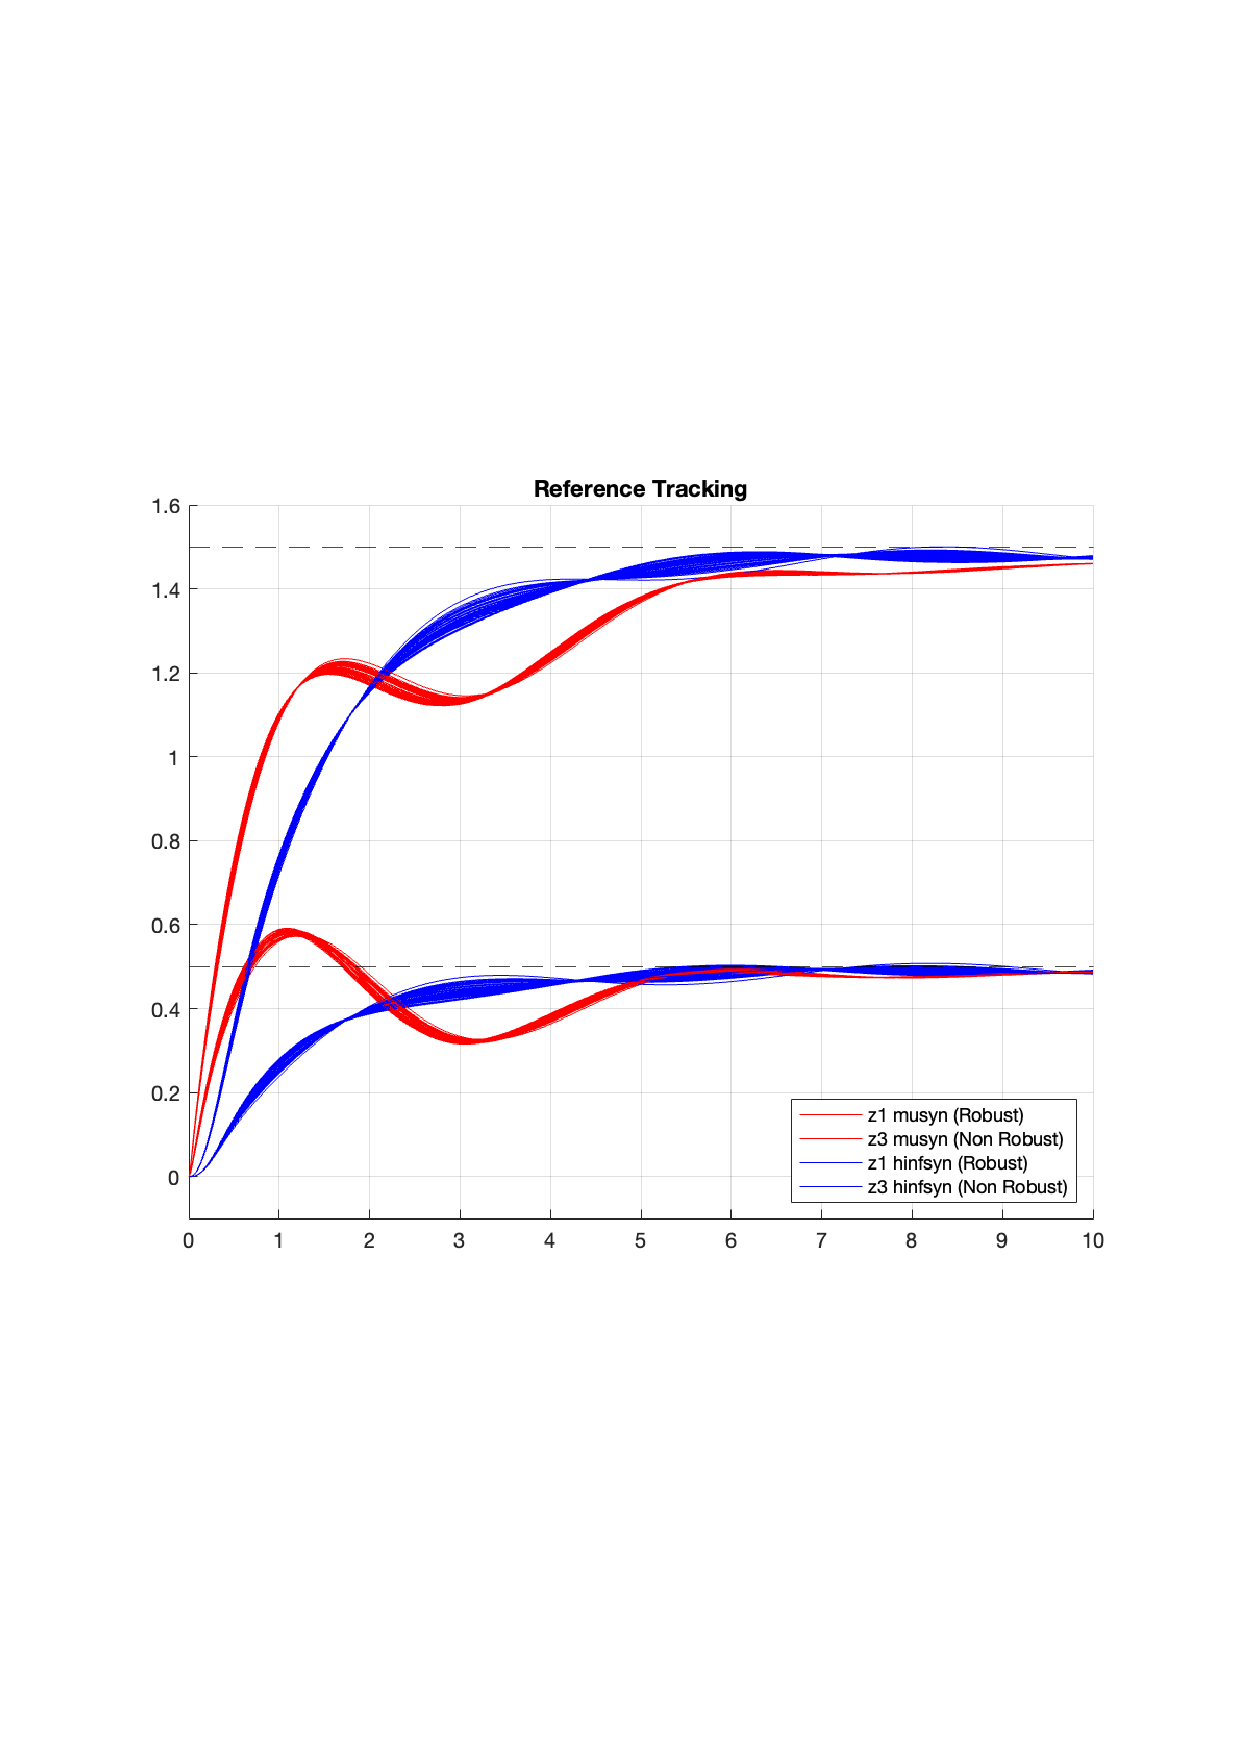
\includegraphics[width=\textwidth]{Figures/fig04a.pdf}
           \subcaption{Reference Tracking Comparison}
           \label{fig:fig04a}
    \end{subfigure}
    \begin{subfigure}[t]{0.45\textwidth}
    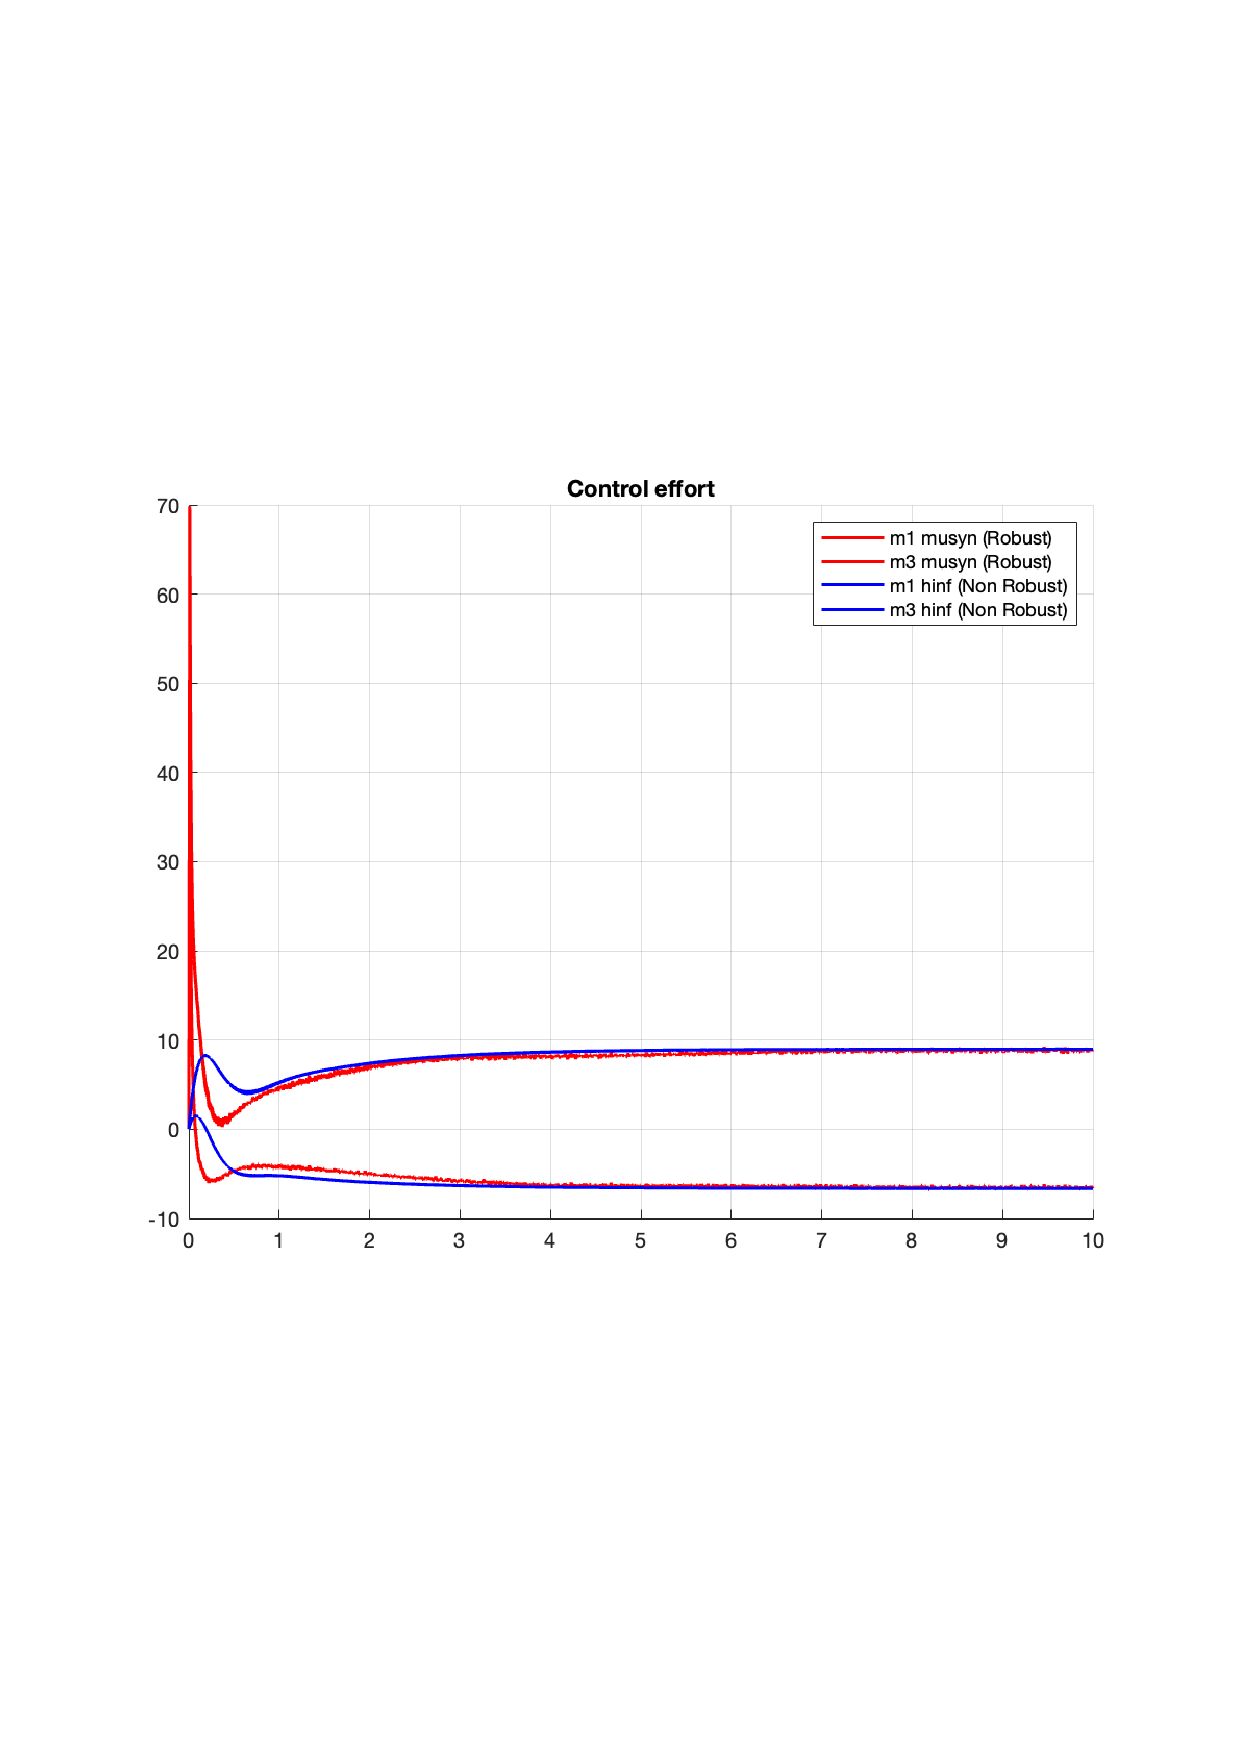
\includegraphics[width=\textwidth]{Figures/fig04b.pdf}
           \subcaption{Control Effort Comparison}
           \label{fig:fig04b}
    \end{subfigure}
    \caption{New $\mu$-synthetized controller vs $hinfsyn$ controller}
    \label{fig:fig04}
   \end{figure}
\\From the plots above, we notice how our "sacrifices" have impacted the system response. The worst "under-performance" comes in terms of control effort: not only the maximum peak in almost 10 times higher, but it's also much more sensitive to measurement noise, exhibiting a pretty evident "sawtooth" outline. 
\\Moreover, the system's response presents some oscillating transient (with a $\approx20\%$ overshoot on the first mass displacement) and a slightly higher tracking error, especially on the third mass.
\section{Problem 2: Transmission Zeros}
In this section, we consider again the same physical system, as for Problem 1, and we want to study the system's transmission zeros and their property depending on the number of Inputs/Outputs chosen.
\subsection{TITO System}
For this case, we consider the  first and second mass to be forced and their relative displacements $z_1,z_2$ to be the measurable variables.
\\\\
We therefore consider
$\begin{bmatrix}
z_1\\
z_2
\end{bmatrix} = 
\begin{bmatrix}
G_{11}(s) & G_{12}(s)\\
G_{21}(s) & G_{22}(s)
\end{bmatrix}
\begin{bmatrix}
f_1\\
f_2
\end{bmatrix}$
to be our TITO system and can then perform the transmission zeros analysis.
\subsubsection{Explicit Calculation}
Being $G(s)$ a square transfer function matrix, we can use a couple of tricks to simplify the computation of the zeros:
\begin{itemize}
    \item Solve $det|G(s)| = 0$ and exclude any solution $z_i$ that is also a pole.
    \item Compute $det|S(s)| = 0$, with $S(s)$ being the system's \textbf{Rosenbrock matrix}  
$S(s) = 
\begin{bmatrix}
sI-A & B\\
C & D
\end{bmatrix}$
\end{itemize}
Useless to say, both solutions are equivalent and give the same result as Matlab's built-in function $tzero(G)$: 
$z_1 \approx -9.81;\ z_2 \approx -20,39$. 
\\ We can also verify the results noticing that both the $G(z_i)$ and $S(z_i)$ matrices drop their rank.
\subsubsection{Zero Input/Output Directions}
We can use the Rosenbrock Matrix $S(s) = 
\begin{bmatrix}
sI-A & B\\
C & D
\end{bmatrix}$ to compute the generalized input direction as a vector that belongs to the null-space of $S(z_i)$, hence:\\ \\
$\xi_z\ state\ vector,\ u_z\ input\ vector\ s.t. \begin{bmatrix}
z_iI-A & B\\
C & D
\end{bmatrix}
\begin{bmatrix}
\xi_z\\
u_z
\end{bmatrix} = 
\begin{bmatrix}
0\\
0
\end{bmatrix}$
\\\\This generalized direction is useful to highlight the \textbf{blocking property of transmission zeros}.
\\This means that, starting from an initial state $x(0) = \xi_z$ and forcing the system with an input $u(t) = u_z e^{zt}$ we obtain an \textbf{identically null output} $y(t) \equiv 0 \ \forall t$.
\\The plots below show the blocking property for both zeros.
\begin{figure}[h!]
    \FigureFive
    \caption{Zero Blocking Property}
    \label{fig:fig05}
\end{figure}
\subsection{TISO system}
Let's now consider a two input one output system, specifically with the first two masses forced by $f_1,f_2$ and the measured output $z_2$.
\subsubsection{Explicit Calculation}
Being the system's transfer function matrix $G(s)$ not square, we can't calculate the determinant of either $G(s)\ or S(s)$.
\\However, to determine when $S(s)$ drops its rank we can calculate (since \#inputs > \#outputs) $det|S(x)S(s)^T| = 0$  and solve for $x$.  
The solutions found are exacly the transmission zeros, which once again are $z_1 \approx -9.81;\ z_2 \approx -20,39$.
\subsubsection{Zero Input/Output Directions}
This time, the null-space of the Rosenbrock matrix $S(z_i)$ is 2-dimensional. Hence we have two generalized input directions that are generators to an invariant subspace. This means that any linear combination of the two generators lies in the invariant subspace and is a "blocking" input vector.\\
\\Calling $u_1,u_2$ the two generators, the relation $S(z_i)(\alpha u_1 + \beta u_2) = 0$ holds $\forall \alpha,\beta$
\\\\
The graph below was generated choosing different linear coefficients for the input generators, both for $z_1$ and $z_2$.
\begin{figure}[h!]
    \FigureSix
    \caption{Zero Blocking Property: TISO}
    \label{fig:fig06}
\end{figure}
\subsection{SITO system}
This time consider a one input two output system, specifically with the first mass forced by $f_1$ and the measured outputs $z_2, z_3$.
\subsubsection{Explicit Calculation}
Once again, the system's transfer function matrix $G(s)$ is not square, but we can determine when $S(s)$ drops its rank.
Since \#inputs < \#outputs) we can calculate $det|S(x)^TS(s)| = 0$  and solve for $x$.  
This time we find only one transmission zero $z_1 = -2$, as also confirmed by Matlab's $tzero(\dots)$.
\subsubsection{Zero Input/Output Directions}
The null-space of the Rosenbrock matrix $S(z_1)$ is again 1-dimensional.\\
Once again, the blocking propery can be visualized also via simulation, with $z_2(t) \equiv 0,\ z_3(t) \equiv 0,\ \forall t$
\begin{figure}[h!]
    \FigureSeven
    \caption{Zero Blocking Property: SITO}
    \label{fig:fig07}
\end{figure}
\clearpage
\section{Problem 3: Decoupling}
Let's go back and consider the same exact system used for both HW03 and HW04. SO far, we faced problems relative to MIMO controller design (often adding some robustness specifications). 
\\\\However, one could think of using decoupling in order to design - instead of a centralized MIMO controller - multiple \textbf{decentralized SISO controllers}.
\\\\
We have different options to perform decoupling, but the main goal remains the same: we want to use a \textbf{decoupling pre-compensator} $D(s)$ that brings us from a general plant (from now on, consider a TITO system) of the kind
$G(s) = \begin{bmatrix}
g_{11}(s) & g_{12}(s)\\
g_{21}(s) & g_{22}(s)
\end{bmatrix}$
to a \textbf{diagonal, apparent plant} of the kind \\
$\Bar{G}(s) := G(s)D(s) = \begin{bmatrix}
\Bar{g}_{11}(s) & 0\\
0 & \Bar{g}_{22}(s)
\end{bmatrix}$.

\subsubsection*{Remark: Need for a preliminary compensator}
Of course one could rule out the need for a decoupling compensator $D(s)$ in presence of an already diagonal system, or still if the anti-diagonal dynamics could be considered neglectable. For instance, in case of off-diagonal terms that have significantly small gain, one could make the choice of ignoring such dynamics and proceed with the decoupled design, being aware of the approximation.
\\
However, for our system, we have the actual need of a compensator, since the two inputs directly effect both outputs significantly. Ignoring the off-diagonal terms would be too big of an approximation and proceeding with the analysis would be pointless.
\subsection{Simplified Decoupling}
Let's now consider the simplest case possible: we want to design $D(s)$ such that the apparent plant is diagonal, with no further requirements whatsoever. 
\\
After that, we can design two decentralized controllers, $C_1(s); C_2(s)$ that stabilize the single control loops with $\Bar{g}_{11}$ and $\Bar{g}_{22}$ respectively.
\\\\
The purpose of the preliminary compensator $D(s)$ is merely canceling out the coupling (off-diagonal) terms of our plant. 
\\
For this reason, we choose 
$D(s) = \begin{bmatrix}
1 & d_{12}\\
d_{21} & 1
\end{bmatrix}$
with $d_{12} = -\frac{g_{12}}{g_{11}}$ and $d_{21} = -\frac{g_{21}}{g_{22}}$.
\\
The resulting decoupled apparent plant is clearly:
\begin{equation}
\Bar{G}(s) = 
\begin{bmatrix}
g_{11}-\frac{g_{21}g_{12}}{g_{22}} & 0\\
0 & g_{22}-\frac{g_{12}g_{21}}{g_{11}}
\end{bmatrix}
\end{equation}
We can therefore perform decoupled control on the two SISO diagonal terms. In this case,we'll use two simple PI controllers to ensure 
exact asympthotic tracking of the desired displacements $r = [0.5, 1.5]^T$.
\\A general control scheme for TITO simplified decoupling can be visualized below
\begin{figure}[h!]
    \FigureEight
    \caption{Simplified Decoupling}
    \label{fig:fig08}
\end{figure}
\\
Simulation results testify a pretty decent behavior of the decoupled system: comparing it with the baseline $H_\infty$ controller designed in HW03, we notice some more oscillating transient but very similar overall performance.
\begin{figure}[h!]
    \FigureNine
    \caption{Simplified Decoupling vs $H_\infty$}
    \label{fig:fig09}
\end{figure}
\subsubsection*{Remark: Preliminary Compensator}
Notice that in our specific case, what the preliminary compensator $D(s)$ is doing is making the force $f_1$ act only on $z_1$ and the force $f_3$ only on $f_3$. It's therefore decoupling what is intrinsically a very "coupled" system, where one force applied strongly affects the movement of all masses.
\subsection{Inverted Decoupling}
Let's now change our design focus a little bit: instead of using $D(s)$ just to make the apparent plant $\Bar{G}(s)$ diagonal, let's try to include some "loopshaping-like" approach to the technique.
\\\\
Let's choose a desired loop function $L_{des}(s) = \begin{bmatrix}
\ell_1^{des}(s) & 0\\
0 & \ell_2^{des}(s)
\end{bmatrix}$.
\\From here, we can use the relationship $L_{des}(s) = G(s)D(s)$ and solve via system inversion: $D(s) := G^{-1}(s)L_{des}(s)$. However, by considering a special structure for $D(s)$ -as a positive feedback of a diagonal matrix with an anti-diagonal one - we can simplify the computations. 
The resulting simulation scheme is reported below:
\begin{figure}[h!]
    \FigureTen
    \caption{Inverted Decoupling Scheme}
    \label{fig:fig10}
\end{figure}
\\The exact implementative choices are left in the Matlab file. What's worth noticing instead is that with inverted decoupling, the controller design in embedded in the loop function assignment. 
\\
\\However, this techniques involves some very "hardcore" cancellations to perform the loop-assignment. Therefore, to consider this a valid choice, the level of "knowledge" of our system must be elevated.
\\\\The more the uncertainty, the less robust this technique become, since not only we might lose the decoupled (diagonal) structure, but also the loop assignment might fail drastically.
\\\\
In the figures below, we notice very good performance obtained through this technique, but again this is not very meaningful if the parameter knowledge is scarce.
\begin{figure}[h!]
    \FigureEleven
    \caption{Inverted Decoupling Simulation Comparison}
    \label{fig:fig11}
\end{figure}
\subsection{Steady State Decoupling: Simplified}
Let's now try to explore if a much "easier" solution still makes the trick. Let's consider again the simplified decoupling scheme, but this time the preliminary compensator will only act at steady state, which means -given the constant reference- at $\omega = 0$.
\\\\
We're looking therefore at a "static" compensator 
$\hat{D} = \begin{bmatrix}
1 & -\frac{g_{12}(0)}{g_{11}(0)}\\
-\frac{g_{21}(0)}{g_{22}(0)} & 1
\end{bmatrix}$. The apparent plant will be diagonal, but only at $\omega = 0$: $\Bar{G}(0) := G(0)\hat{D} = \begin{bmatrix}
\Bar{g}_{11}(0) & 0\\
0 & \Bar{g}_{22}(0)
\end{bmatrix}$.
\\\\This method highlights what are the complications that arise from the intrinsically "highly coupled" nature of the system: the off-diagonal terms are only compensated at steady-state, but they actually deeply affect the response in the transient.
\\For this reason, it's no surprise that the steady-state decoupled system, using the same PI decentralized controllers, is unstable, as shown in the graph below.
\begin{figure}[h!]
    \FigureTwelve
    \caption{Unstable system under Steady State Simplified Decoupling}
    \label{fig:fig12}
\end{figure}
\subsection{Sequential Loop Closure}
Let's now try, for the first time so far, a "pure" decentralized control technique, that doesn't rely at all on compensators.
\\\\
The idea behind sequential loop closure is selecting an input-output pair - in our case $z_3 = g_{22}(s)f_3$ - (ignoring all the others) and design a controller for just that "channel". 
\\\\
After that, we must close the channel's loop and design another controller on the remaining channel, - $z_1 = g_{11}(s)f_1$ - but taking into account the lower loop. 
\\\\
This procedure doesn't need any form of compensation and utilized only the two SISO controllers designed as for above. In particular, the chosen controllers were PIDs designed through the Matlab $pidtune(\dots)$ command, with a design focus on reference tracking.
\\\\
Simulation result show how this control technique offers the worst performance so far, with a close to 100\% overshoot on the output $z1$. Of course one could try to better tune the PID controllers to mitigate this under-performance, but it's still indicative of the fact that with no kind of pre-compensation, the achieved performance decays. On the flip side, not relying on exact compensation is still a wise choice in case of uncertainty.
\begin{figure}[h!]
    \FigureThirteen
    \caption{Sequential Loop Closure Response (2 PID controllers)}
    \label{fig:fig12}
\end{figure}

\clearpage
\section{Problem 4: Limitations}
Let's now consider a totally different system, namely
\begin{equation}
G_{NMP} = \frac{1}{(s+10)(s+2)}
\begin{bmatrix}
(s-2) & (s+1)\\
(s+1) & (s-2)
\end{bmatrix}
\end{equation}
The plant admits a minimal realization of the kind 
$A = \begin{bmatrix}
-12  &  -5  &   0  &   0 \\
 4   &  0   &  0   &  0 \\
 0   &  0   &-12   & -5 \\
 0   &  0   &  4   &  0 \\
\end{bmatrix}$;
$B = \begin{bmatrix}
2  &   0 \\
0  &   0 \\
0  &   2 \\
0  &   0 
\end{bmatrix}$;
$C = \begin{bmatrix}
0.5 &-0.25  & 0.5  & 0.125 \\
0.5 &  0.125 &  0.5 & -0.25
\end{bmatrix}$;
$D = \begin{bmatrix}
0 & 0 \\
0 & 0
\end{bmatrix}$;
\\ From there, we can find the transmission zeros solving $det|S(s)| = 0$, with $S(s)$ being the system's \textbf{Rosenbrock matrix}.
\\\\
It turns out the system has only \textbf{one transmission zero in z = 0.5}. 
\\ Notice however that the diagonal input-output channels (SISO) have also a NMP zero in $z_i = 2$. This can be a problem when facing decoupling.
\subsection{Simplified Decoupling Limitationa}
Before we dig into performance limitations, let's first consider the same preliminary compensator we used before, which is $D(s) = \begin{bmatrix}
1 & d_{12}\\
d_{21} & 1
\end{bmatrix}$
with $d_{12} = -\frac{g_{12}}{g_{11}}$ and $d_{21} = -\frac{g_{21}}{g_{22}}$. Using such a compensator would be a great mistake, since both the diagonal terms $g_{11}, g_{22}$ present a n.m.p. zero and their inversion leads to the introduction of unstable poles.
\\\\
For this exact reason, we're going to use a different type of compensator, which is $D'(s) = \begin{bmatrix}
d_{11} & 1\\
1 & d_{22}
\end{bmatrix}$
with $d_{11} = -\frac{g_{22}}{g_{21}}$ and $d_{22} = -\frac{g_{11}}{g_{12}}$.\\
This choice leads to an apparent plant 
\begin{equation}
\Bar{G}(s) := G(s)D'(s) = \begin{bmatrix}
\frac{6(s-0.5)}{(s+10) (s+2) (s+1)} & 0\\
0 & \frac{6(s-0.5)}{(s+10) (s+2) (s+1)}
\end{bmatrix}
\end{equation}
We notice that the transmission zero appears in both I/O channels and it's clear that no unstable cancellation happened. Moreover, since the two decoupled channels have the same dynamics, we can define two identical controllers to achieve the exact same performance on both.
\subsubsection{Performance Limitations}
Let's now try some $H_\infty$ design to add some specifications on the system's reference tracking. Assume we want to assign a constant unitary reference to each input channel and want to keep the tracking error under 1\%.
\\\\
We try two different sensitivity weight functions ($w_S_1, w_S_2$) with the same shapes but different bandwidth ($B_{3S_1} = 0.2, B_{3S_2} = 1$). We'll also try to limit control effort with a constant $w_u = 0.01$. 
\\\\
After, synthetizing the controllers using $mixsyn(\dots)$ and the weights just defined, we can calculate the SISO sensitivity functions $S_1(s), S_2(s)$.
\\The plot below testifies the well known \textbf{waterbed effect}, where pushing bandwidth causes an increase of "positive area" that will strongly affect performance, due to the sensitivity peaks.
\begin{figure}[h!]
    \FigureFourteen
    \caption{Waterbed Effect on Sensitivities}
    \label{fig:fig14}
\end{figure}
\subsection{MIMO Design}
To evaluate the results obtained with decoupling, we can try to perform MIMO design, this time using 2x2 diagonal weights, whose diagonal elements are the same exact weights designed above.
\\\\
The plot in the next page shows how the achieved performance is very similar to the decoupled case. The common denominator is however the undershoot due to the non-minimum-phase zero. Notice however how increasing bandwidth leads to huge undershoots, up to -200\%. Therefore, we can conclude that settling for a slower response is the only way to cope with the limitations introduced by the NMP zero.
\begin{figure}[h!]
    \FigureFifteen
    \caption{Decoupled vs MIMO response: greedy vs compromise controllers}
    \label{fig:fig15}
\end{figure}
\end{document}